%%%%%%%%%%%%%%%%%%%%%%%%%%%%%%%%%%%%%%%%%%%%%%%%%%%%%%%%%%%%%%%%%%%%%%%%%%%%%
%%
%% This file provides a template that can be used in concert with the
%% ohio-etd class to generate an electronic thesis or dissertation which
%% meets the formatting requirements at Ohio University.
%%
%% To use the template, copy this file (template.tex) and ohio-etd.cls into
%% the same directory and edit this template as required.  Reference
%% ohio-etd.pdf for additional instructions on using this class.
%%
%%%%%%%%%%%%%%%%%%%%%%%%%%%%%%%%%%%%%%%%%%%%%%%%%%%%%%%%%%%%%%%%%%%%%%%%%%%%%


%% Load the class.  Available options are: numbered, pdftex, cmfont,
%% singlespacetables, draft, 11pt, 12pt, leqno, and fleqn

\documentclass[numbered,pdftex]{ohio-etd}
\usepackage{cite}
\usepackage{notoccite}
\usepackage{bbding}
\usepackage[utf8]{inputenc}



\usepackage[normalem]{ulem}

\usepackage{ragged2e}
\usepackage{verbatim} 
\usepackage{hyperref}
\usepackage{flafter}
\usepackage{color,soul} % Highlighting 
\usepackage{subfigmat}

\usepackage{float} % In-text figs
\usepackage{varioref}%  smart page, figure, table, and equation ref
\usepackage{graphicx} % Include graphics
\usepackage{epstopdf} % Figure type .eps to .pdf
\usepackage{wrapfig} % Figures in text
\usepackage{listings}
\usepackage{color} %red, green, blue, yellow, cyan, magenta, black, white

\floatstyle{boxed}
\restylefloat{figure}


\definecolor{mygreen}{RGB}{28,172,0} % color values Red, Green, Blue
\definecolor{mylilas}{RGB}{170,55,241}


%% Other packages that may be of use.  Delete or comment out (using a
%% percent sign in the first column) if they are not desired.  Reference
%% the corresponding documentation for more information on how to use these
%% packages.

%\usepackage[square,sort&compress,numbers]{natbib} % Provides formatting for
                                                  % citations
\usepackage{textcomp} % Provides math symbols that can be used in text mode
\usepackage{amssymb}  % Provides additional AMS math symbols.  Note that
                      % amsmath is loaded as part of the ohio-etd class
\usepackage{bm}       % Provides bold-faced math symbols
\usepackage{booktabs} % Provides improved table formatting
\usepackage{dcolumn}  % Provides table columns aligned at decimal points
\usepackage{multirow} % Provides table elements spanning multiple rows
\usepackage{graphicx} % Standard package to incorporate graphics
\usepackage[printonlyused]{acronym} % Provides a method for incorporating
                                    % acronyms and building an acronym list
\usepackage{relsize}
\usepackage{amsmath} % Inserting Equations

\graphicspath{{figures/}} % Allows graphics files to be stored in a
                          % separate directory
\usepackage{fancyref}
\usepackage{}

%% Required front matter definitions

\degree    {MS}              % MS, MA, MCTP, or PhD
\graduation{May}{2018}    % May, August, or December 

\title     {A Proposal for a Parameterized Circulating Vector Field Guidance for Fixed Wing Unmanned Aerial Vehicles}
\author    {Garrett S.}{Clem} 

\advisor   {Jay P. Wilhelm}{Assistant Professor of Mechanical Engineering}
\dean      {Dennis Irwin}{Dean, Russ College of Engineering and Technology }
\program   {Mechanical Engineering}            % e.g. Electrical Engineering
\department{Department of Mechanical Engineering} % e.g. School of Electrical Engineering 
                                    %      and Computer Science
\college   {Russ College of Engineering and Technology}   % e.g. Russ College of Engineering and
                                     %      Technology
\abstract  {Unmanned Aerial Vehicles (UAVs) are guided to fly along straight line obstacle free paths that connect pre-planned waypoints. Initially undiscovered obstacles encountered during flight may require waypoints to be re-planned. Obstacles could be avoided without the need to re-plan mission waypoints by implementing vector field path following in conjunction with repulsive obstacle vector fields. Repulsive vector fields that combine weighted repulsive and attractive components to provide an optimal obstacle avoidance guidance will be investigated to avoid singularities and improve path tracking performance compared to waypoint guidance.}
 

%% Optional front matter definitions.  Delete or comment out if not needed

% \coadvisor {Coadvisor's Full Name}{Coadvisor's Full Title}

%\dedication{DED}
%
%\acknowledgments{ACK}
%% If you prefer to provide "acknowledgements" instead (note the added "e"
%% between the "g" and the "m") then add the "e" in the macro name so that
%% it reads "\acknowledgements".}

%% Additional "lists" can be added to the end of the front matter using the
%% \addlistof macro.  For example:
\addlistof{Symbols}{\begin{tabbing}
  XXXXXXXXXXXX \= \kill% this line sets tab stop
  \\
  $\vec{v} $ \> Vector field \\
  $\vec{v}_{conv}$ \> Convergence component \\
  $ \vec{v}_{circ}$ \> Circulation component \\
  $ \vec{v}_{tv}$ \> Time-varying component \\
  $G$ \>Convergence weight  \\
  $H$ \>Circulation weight  \\
  $L$ \>Time-varying weight  \\
  $q$ \>Spatial dimension set  \\
  $\alpha_i(x_1,x_2,...x_n,t)$ \> Implicit surface function \\
  $n$ \> Number of spatial dimensions \\
  $t$ \>Time  \\
  $i$ \>index \\
  $\nabla_q$ \>Gradient with respect to spatial dimensions q  \\
  $M$ \>Gradient matrix  \\
  $a$ \>Velocity column vector  \\
  $\vec{V}$ \>Total field  \\
  $d$ \>Range  \\
  $P$ \>Decay weight  \\
  $R$ \>Radius  \\
  $\vec{v}_{repulsive}$ \>Repulsive vector field  \\
  $\vec{v}_{attractive}$ \>Attractive vector field \\
  $u$ \>Speed  \\
  
  
  
  
  

 \end{tabbing}}
%% Note that the command "\input{symbols}" can be used if the symbol list is
%% contained in a separate file called "symbols.tex"}

\addlistof{Acronyms}{

\begin{tabular}{lll}
UAV & Unmanned Aerial Vehicles & \\
VF & Vector Field & \\
UAS & Unmanned Aerial System  & \\
VFF & Virtual Force Field  & \\
TPLVF & Tangent Plus Lyapunov Vector Field & \\
RRT* & Optimal Rapid Radom Trees & \\
DT  & Delauny Triangulation & \\
GVF & Gradient Vector Field & \\
 
\end{tabular}}


%% Use "\input{acronyms}" if the acronym list is in a separate file called
%% "acronyms.tex".  Note that the formatting generated by the acronym package
%% can be forced into singlespaced text by inserting "\setlength\itemsep{0pt}
%% \setlength\parskip{0pt}" into the "acronym" environment.} 

%% For documents created by government employees as part of their
%% employment.  The wording of the disclaimer can be specified using an
%% option.  See the documentation for more information.

% \govtdisclaimer    

\notables  % Prevent a list of tables from being created
% \nofigures % Prevent a list of figures from being created

\begin{document}

\makefrontmatter    % Creates all of the front matter pages.

% for matlab code entrys
\lstset{language=Matlab,%
    %basicstyle=\color{red},
    breaklines=true,%
    morekeywords={matlab2tikz},
    keywordstyle=\color{blue},%
    morekeywords=[2]{1}, keywordstyle=[2]{\color{black}},
    identifierstyle=\color{black},%
    stringstyle=\color{mylilas},
    commentstyle=\color{mygreen},%
    showstringspaces=false,%without this there will be a symbol in the places where there is a space
%     numbers=left,%
%     numberstyle={\tiny \color{black}},% size of the numbers
%     numbersep=6pt, % this defines how far the numbers are from the text
    emph=[1]{for,end,break},emphstyle=[1]\color{red}, %some words to emphasise
    %emph=[2]{word1,word2}, emphstyle=[2]{style},    
}

%% Body of the text follows, using \chapter, \section, \subsection,
%% \subsubsection, \paragraph, and \subparagraph to generate the
%% section headings.  For convenience, it may be useful to break the
%% full document into separate files, perhaps divided by chapters.  In
%% that case, the files would be loaded here using "\input{filename}"


 \chapter{Introduction}
\section{Motivation and Problem Statement}

%Fixed wing Unmanned Aerial Vehicles are used for missions such as surveillance and reconnaissance that might put pilots harm’s way \cite{bone_uavs_2003}. Missions consist of sequential objectives that are represented by a path that the UAV attempts to follow. Paths are typically pre-planned before flight and are constructed by connecting straight lines and circular arcs. Vehicle turn rate constraints and obstacles are considered when planning a path to prevent collisions or entry into no-fly zones. UAVs are guided to follow a path by implementing guidance algorithms which calculate headings that minimize the distance to a path. UAVs may encounter an obstacle whose position was previously unknown while following a pre-planned path which may require a new path to be generated. Guidance that follows mission paths while avoiding obstacles without the need for re-planning may be beneficial. 
%\\
%Gradient Vector Field (GVF) guidance is a path following method that has been adapted for obstacle avoidance. GVFs produces continuous heading vectors that guide a UAV to converge and follow a path by summing together convergence and circulating terms that are weighted by static scalars. An obstacle represented as a path and given a negative convergence weight results in a repulsive field that can be used for obstacle avoidance. Static GVFs do not always route the UAV around an obstacle and could be improved. Modifying the GVF convergence and circulation weights of obstacle fields to be functions of common UAV states could be used to produce an optimal guidance for obstacle avoidance. \textbf{The proposed research seeks to determine GVF weighting functions that construct optimal obstacle avoidance.}
Fixed wing Unmanned Aerial Vehicles (UAVs) are used for missions such as surveillance and reconnaissance that might put pilots in harm’s way \cite{bone_uavs_2003}. Missions typically consist of sequential objectives represented as waypoints that the UAV follows. Waypoints may be pre-planned before flight where vehicle constraints and obstacles can be considered to prevent collisions or entry into no-fly zones. UAVs follow waypoints by implementing guidance algorithms that calculate headings to direct a UAV along a path connecting the waypoints. Obstacles may be discovered during flight that were unknown at initial planning and a new set of waypoints may have to be generated.  Waypoints are typically computed at a ground station and are relayed to the UAV by radio, which may be problematic if communication with the UAV is lost. Guidance that accomplishes mission objectives while avoiding obstacles without the need for re-planning waypoints may be beneficial. 
\\
Vector Field (VF) guidance is a method that is mainly used for path following and can be useful for obstacle avoidance \cite{wwc,panagou_motion_2014}. VFs can produce continuous heading vectors that can be used to guide a UAV to coverage and follow a path. Vectors are calculated by summing together convergence and circulation terms that are weighted by static scalars. Obstacles can be represented as a path and given a negative convergence weight resulting in a repulsive field. Static repulsive VFs do not always route the UAV around an obstacle. Modifying repulsive VF parameters to be functions of common UAV states may be used to produce an optimal guidance. \textbf{The proposed research seeks to determine VF weighting functions that enable optimal obstacle avoidance.}



 \pagebreak
 
 \section{Methods Overview}
 
 The proposed research was conducted in three phases consisting of numerical simulations and indoor flight experiments. Phase I consisted of demonstrating and numerically locating VF guidance singularities in a summed vector field. Static repulsive field weights and decay radius were investigated and optimized to produce minimal path deviation using VF guidance in simulation in Phase II. Lastly, flight experiments using a indoor flying quadcopter using the optimized VF guidance under fixed-wing UAV constraints was conducted. 
 
% The proposed research will be conducted in three phases where VF guidance  singularities will be demonstrated, weighting functions  that influence obstacle avoidance will be investigated, and a optimized GVF will be validated on a crazyflie quadcopter simulating fixed wing UAV constraints.  Phases I and II will be conducted in a simulation environment that combines mission paths and obstacles into a single GVF. Phase III will be conducted with a quadcopter flying at constant altitude emulating a fixed wing UAV guided by the modified GVF in real-time. Dubin's fixed wing constraints will be imposed in simulations and experiments. 
% 

 \section{Phase I}
 \textbf{Characterize and present a method for locating singularities in a summed GVF.} A simulation environment will be built that generates GVFs consisting of mission paths and obstacles. Circular obstacles will be investigated and the resulting singularities will be characterized. Static weights will be used and the performance of the guidance measured in distance traveled and time of flight. 
 
 
 
 \section{Phase II}
 \textbf{Determine a combination of circulation and decay radius for a circular obstacle GVF that produces an optimized obstacle avoidance.} UAV closing rate, position, and range will be used to develop dynamic GVF weights for convergence and circulation. The modified GVF will be compared against a static and strictly repulsive GVF. Distance traveled and time of flight will be used to as metrics to compare the modified GVF to the unmodified GVF.  
 
 
 
 \section{Phase III}
 \textbf{Demonstrate optimized GVF guidance on multirotor UAV flying with fixed wing turn-rate constraints.} The modified GVF developed in Phase II will be implemented on a differential multirotor UAV emulating a fixed wing UAV Dubins constraints. Guidance performance while avoiding static circular obstacles will be demonstrated.
 
 
 \section{Summary of Objectives}
 
 Each phase consists of an \textbf{objective} that was accomplished by executing several \textit{tasks}.
 Completion of all objectives and phases will result in the final \underline{deliverable}. \\[1cm]
 
 \noindent
 \textbf{Phase I Objective:} Demonstrate and locate singularities in a summed gradient vector field
 \newline
 \textit{
 	Tasks:
 	\begin{enumerate}
 		\item Build a GVF simulation environment
 		\item Evaluate scenarios where singularities are expected
 		\item Characterize location of singularities 
 	\end{enumerate}
 }
 
 \noindent
 \textbf{Phase II Objective:} Determine combination of repulsive gradient vector field circulation and decay radius that minimizes path deviation
 \newline
 \textit{
 	Tasks:
 	\begin{enumerate}
 		\item Formulate circulation and convergence weights as functions of UAV state
 		\item Determine combination of GVF weights that produces optimal guidance in simulation
 	\end{enumerate}
 }
 
 \noindent
 \textbf{Phase III Objective:} Validate modified gradient vector field guidance with indoor quadrotor experiments
 \newline
 \textit{
 	Tasks:
 	\begin{enumerate}
 		\item Build differential drive robot
 		\item Build robotic framework to take guidance commands
 		\item Repeat simulations performed in Phase II on ground robot
 	\end{enumerate}
 }
 
 \noindent
 \textbf{Deliverable:} \underline{Adaptive GVF parameterized weights optimal guidance for path following and static} \underline{ obstacle avoidance}.
 
 





\chapter{Literature Review}
\section{Literature Review Introduction}


%Essentially what is inside of literature review
%
%- UAVs and the framework that allows them to operate\\
%- / how they are integrated with other support systems (UAS)\\
%- Tasks and how they are typically carried out (path following / waypoint guidance)\\
%- Something about obstacles and the need for re-planning\\
%- Guidance systems that do not require re-planning and issues involved in their use\\


\section{Unmanned Aerial Vehicles}
Unmanned aerial vehicles (UAVs) are gaining popularity in military and civilian communities for their ability to autonomously perform tasks such as data collection, target tracking, and package delivery. In general, UAVs are categorized into fixed wing and rotor craft varieties \cite{beard_small_2012} that range in size, payload, and flight time capabilities. Fixed wing UAVs (Figure \ref{fig:fixedMultirotor}a) are typically used for tasks that require larger payloads, such as cameras and cargo, and longer flight times. Multirotor UAVs (Figure \ref{fig:fixedMultirotor}b), in general, have lower payload capabilities compared to fixed wing UAVs, however do not require a large clearing for takeoff and landing and have a small turning radius making them more maneuverable.

\begin{figure}[H]
	\begin{subfigmatrix}{2}% number of columns
		\centering	
		\subfigure []{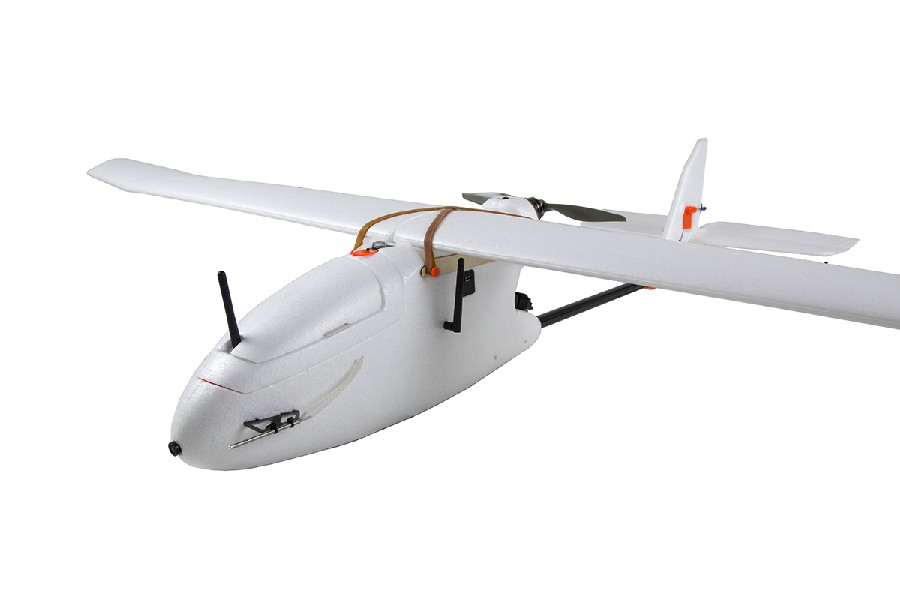
\includegraphics[width=6.5cm,trim=0 0 0 0,clip] {PaperFigures/fixedwing}}
		\subfigure []{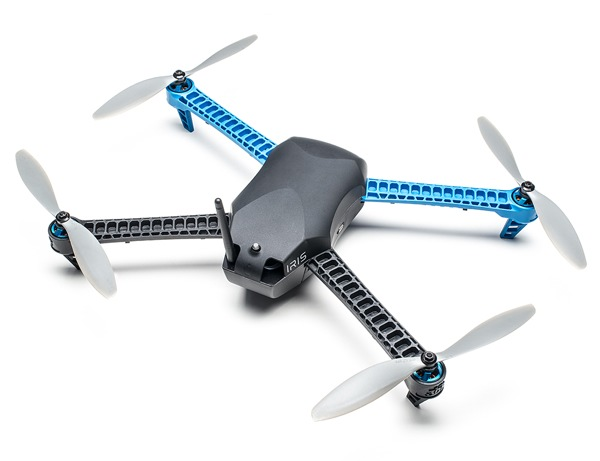
\includegraphics[width=6.5cm,trim=0 0 0 0,clip] {PaperFigures/iris-1}}
		\hspace*{0mm}
	\end{subfigmatrix}
	\caption{Fixed wing (a) and multirotor (b) UAVs}
	\label{fig:fixedMultirotor}
\end{figure}

Using UAVs has several advantages over manned aircraft consisting of low operating cost, reduced risk to human operators, and the ability to perform mundane and repetitive tasks autonomously without heavy human interaction. Open source and versatile autopilots developed by a world-wide community of hobbyist and professionals have made UAV technology widely available on relatively inexpensive hardware [pixhawk, ardupilot]. UAVs can be piloted remotely, removing pilots from potentially dangerous situations if an aircraft experiences mechanical failure. The power behind UAVs lies in their ability to be programmed to carry out tasks autonomously and with little human interaction, allowing operators to monitor multiple vehicles simultaneously. Tasks may be carried out by a single UAV or in cooperation other air or ground vehicles \cite{oh_coordinated_2013,hyondong_oh_coordinated_2015,ulun_coordinated_2013}. The aircraft's route can be controlled directly by an operator's radio controller input when the vehicle is within line-of-sight (LOS). For long endurance or beyond LOS missions, the UAV can be programmed to autonomously follow a mission path that is typically generated prior to flight on a dedicated ground station. Flying autonomous missions typically requires not only the UAV and the autopilot, but a ground support station and hardware to communicate with the ground. 

 \begin{figure}[H]
	\centering
	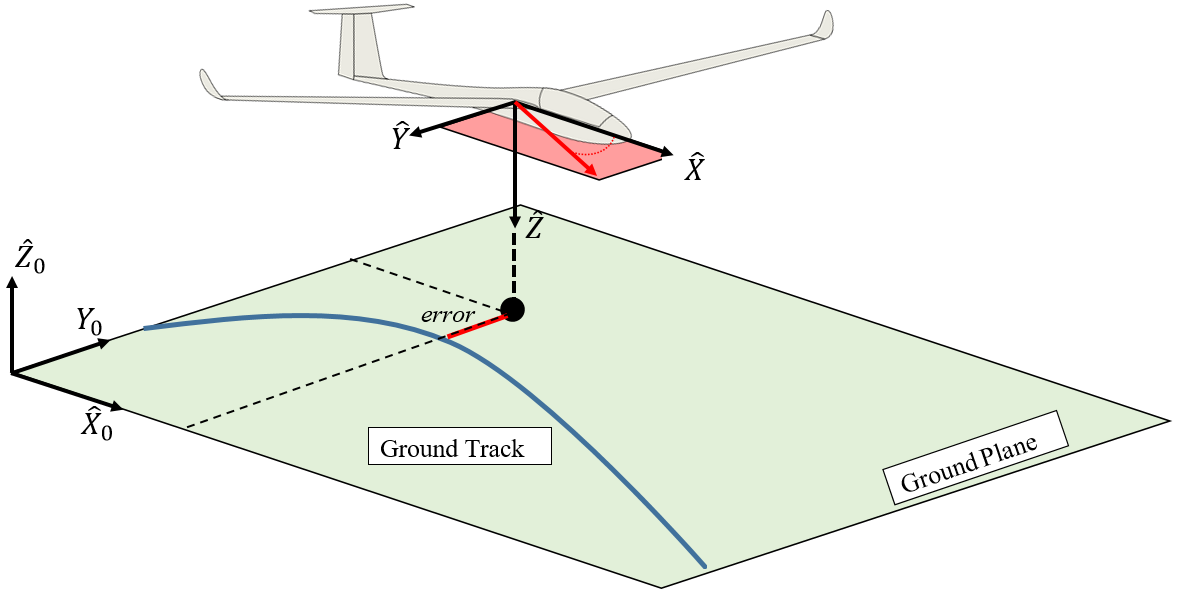
\includegraphics[width=12cm]{PaperFigures/UAVFrame}
	\caption{}
	\label{fig:uavframe}
\end{figure}
%The UAV, ground station, and communication hardware is referred to as an unmanned aerial system (UAS).


\section{Unmanned Aerial Systems (UAS)}
These UAVs and autopilots are part of an Unmanned Aerial System (UAS) which work in conjunction with ground stations, radio control transmitters, and two way radios. The UAV craft provides the support structure, lifting and control surfaces, and housing for the autopilot, radios, and sensors. Ground stations are responsible for monitoring the vehicle's status, planning missions, and generating obstacle free and flyable paths which are sent to the autopilot via two way radio.


\subsection{Ground Stations}
Ground stations are the hardware and software framework used to configure UAV settings, plan missions, and collect mission data. Commercial open source ground stations such as qground control depend on a human operator's knowledge of the environment to plan an obstacle free path. Takeoff, landing, and emergency return-to-home locations are designated in safe clearings capable of accommodating the vehicle. Other tasks such as area surveying and loitering can be assigned at certain points along the mission path. An example of a mission consisting of taking off, surveying, and landing is shown in Figure \ref{fig:groundstationplanning}




\begin{figure}[H]
	\centering
	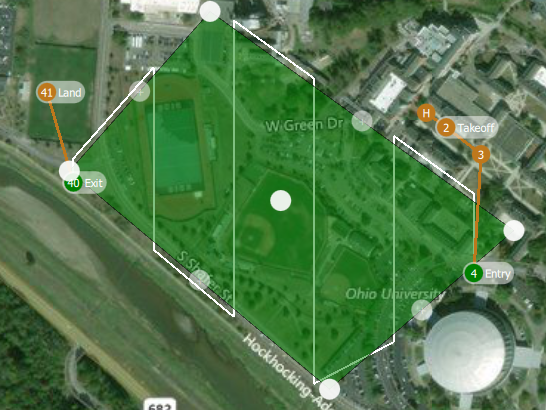
\includegraphics[width=12cm]{PaperFigures/Literature/groundStationPlanning}
	\caption{Ground station software planning a waypoint based mission}
	\label{fig:groundstationplanning}
\end{figure}

Mission paths are typically represented as a series of finite waypoints that are relayed to the UAV over radio where an on-board guidance system interprets them.\\

====================\\
Obstacle free and flyable paths are typically pre-planned and generated off-line at a dedicated ground station using a path planner. Many methods can be used for generating paths, however the process is generally executed in two steps consisting of optimization and refinement. Optimization builds shortest path taking in constraints such as obstacles and mission objectives. The optimized path is then refined to meet a vehicles dynamic constraints, such as turn rate and velocity. \\
=====================\\

\subsection{Autopilot}
The UAV autopilot is responsible for controlling a pre-planned path and maintaining vehicle stability while under the influence of external wind disturbances. Stable flight while path following is accomplished by implementing feed-back control, navigation, and guidance systems. A high level overview of the autopilots systems can be seen in Figure \ref{fig:autopilotloops}. Feed-back refers to the closure of an open-loop control system which allows a reference error to be calculated between the desired state of the UAV, the reference, and the current state of the UAV. Reference error is used to calculate the necessary actuator output required to modify the vehicles attitude and position while preventing unbounded oscillation. Attitude and position feed-back is provided by the navigation system by sampling on-board sensors such as global position system (GPS) and inertial measurement units (IMUs). Filtering and fusing noisy data from multiple sources is often accomplished through estimation techniques such as the Kalman filter. \\



%\begin{figure}
%	\centering
%	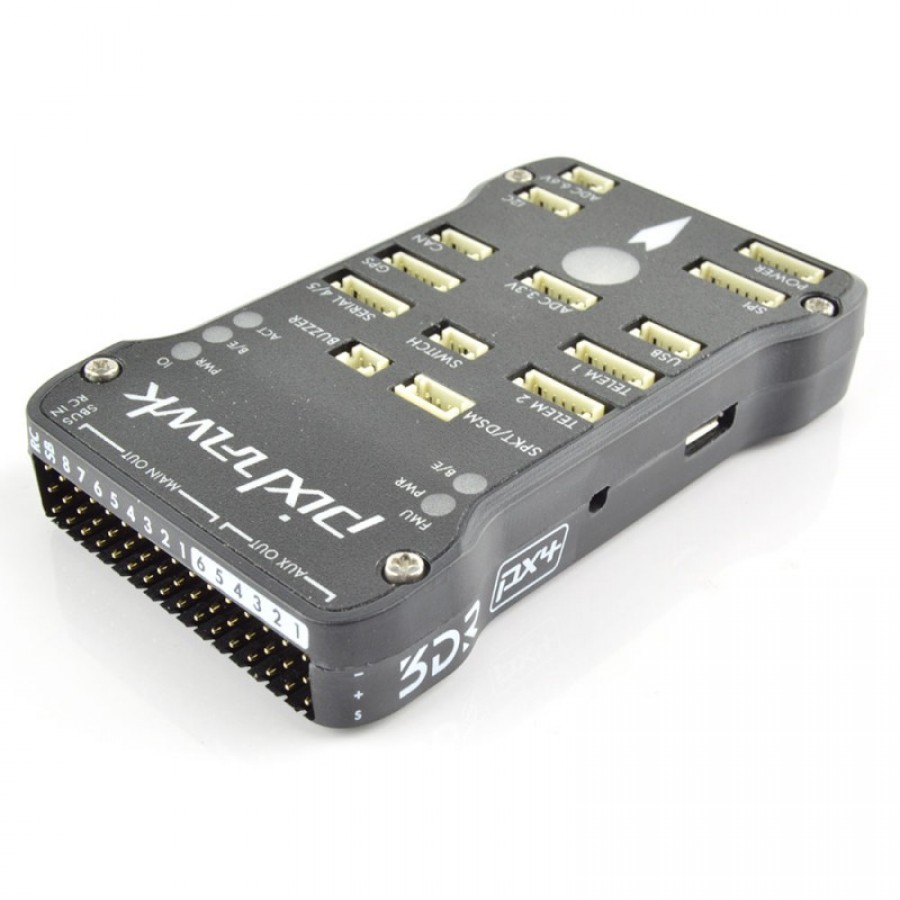
\includegraphics[width=8cm]{PaperFigures/pixhawk}
%	\caption{Pixhawk autopilot}
%	\label{fig:pixhawk}
%\end{figure}
%
%
%



%\begin{figure}
%	\centering
%	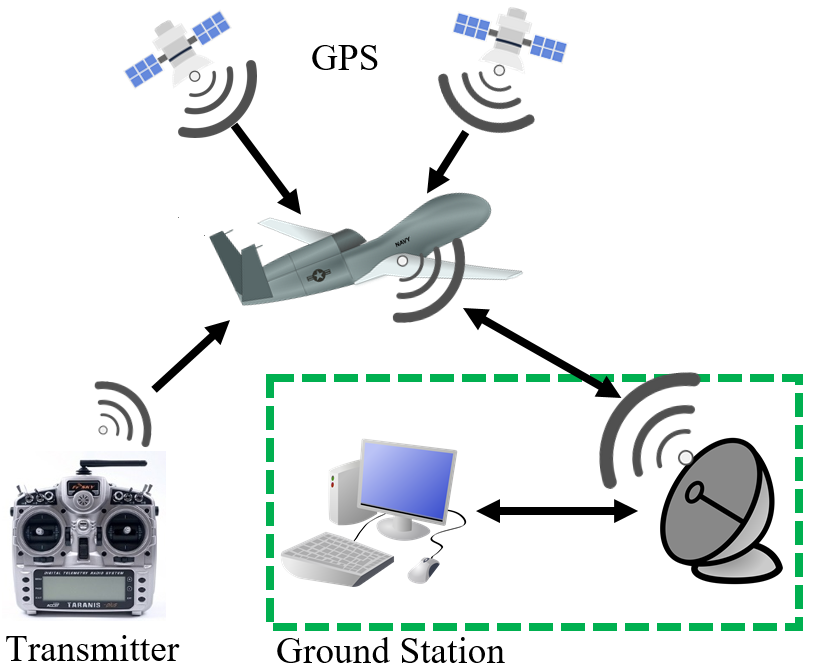
\includegraphics[width=12cm]{PaperFigures/UAS}
%	\caption{Unmanned Aerial System (UAS)}
%	\label{fig:uas}
%\end{figure}

\begin{figure}
	\centering
	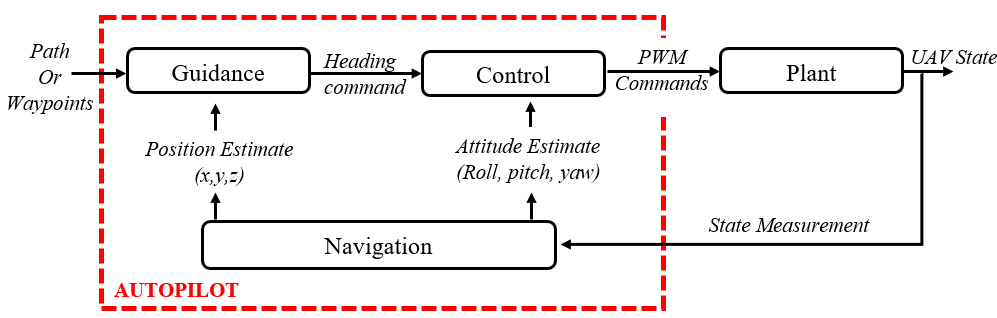
\includegraphics[width=15cm]{PaperFigures/autopilotLoops2}
	\caption{Autopilot's Navigation, Guidance, and Control Architecture}
	\label{fig:autopilotloops}
\end{figure}

\section{UAV Guidance}
On-board guidance systems attempt to minimize the lateral error to the path by commanding a heading pointing to the path. Guidance methods for following a pre-planned path include geometric methods such as waypoint or carrot chasing and control techniques such as proportional-integral-derivative (PID), non-linear guidance laws, and linear quadratic regulator (LQR) \cite{sujit_unmanned_2014}. Due to traditional guidance method's dependence on a path planner to construct an obstacle free and flyable path, these methods often lack a mechanism to avoid new obstacles. Re-planning and relaying a new obstacle free path may be impossible under certain conditions, such as flying beyond line-of-sight. Path planning on-board to avoid a new obstacle could be accomplished by inserting a new temporary path or by completely re-planning, however introduces several challenges such as waypoint placement and density. It would be beneficial to include obstacle avoidance into a UAVs guidance system to remove the need to communicate with the ground station or use an on-board path planner which may be accomplished with potential field or vector field. \\


%\subsection{Waypoint Guidance}
%Waypoint guidance aligns the vehicle with the current active waypoint that lies along a pre-planned path. Paths are typically generated off-line and can be optimized for shortest distance traveled and further refined to be flyable for a particular vehicle. Paths may also be optimized to produce flight patterns that increase sensor coverage of an area of interest \cite{wilhelm_direct_2017}. 
%
%If an obstacle lies along that sensor path, the UAV must avoid the obstacle but also return back to the sensor path such that a minimal length of the path is missed during data collection. The number of waypoints that divert around an obstacle effects how closely the UAV tracks the outside of the obstacle and how much of the original path can be traveled. Few obstacle diversion waypoints leads to excess path deviation. Increasing the number of diversion waypoints reduces path deviation, however has diminishing returns. A cost function $\gamma$ can be used to measure the deviation from a planned path while avoiding obstacles with diversion waypoints, shown in Equation \ref{eq:diversionCost}.
%
%\begin{equation}
%\label{eq:diversionCost}
%\begin{aligned}
%\gamma =  \frac{1}{r_O}\int_{0}^{tf}ydt
%\end{aligned}
%\end{equation}
%
%
%An example of a UAV following diversion waypoints is shown in Figure \ref{fig:numWaypointsPath} and the cost associated with increasing number of waypoints in Figure \ref{fig:numWaypoints}.
%
%
%\begin{figure}[H]
%	\begin{subfigmatrix}{2}% number of columns
%		\centering	
%		\subfigure []{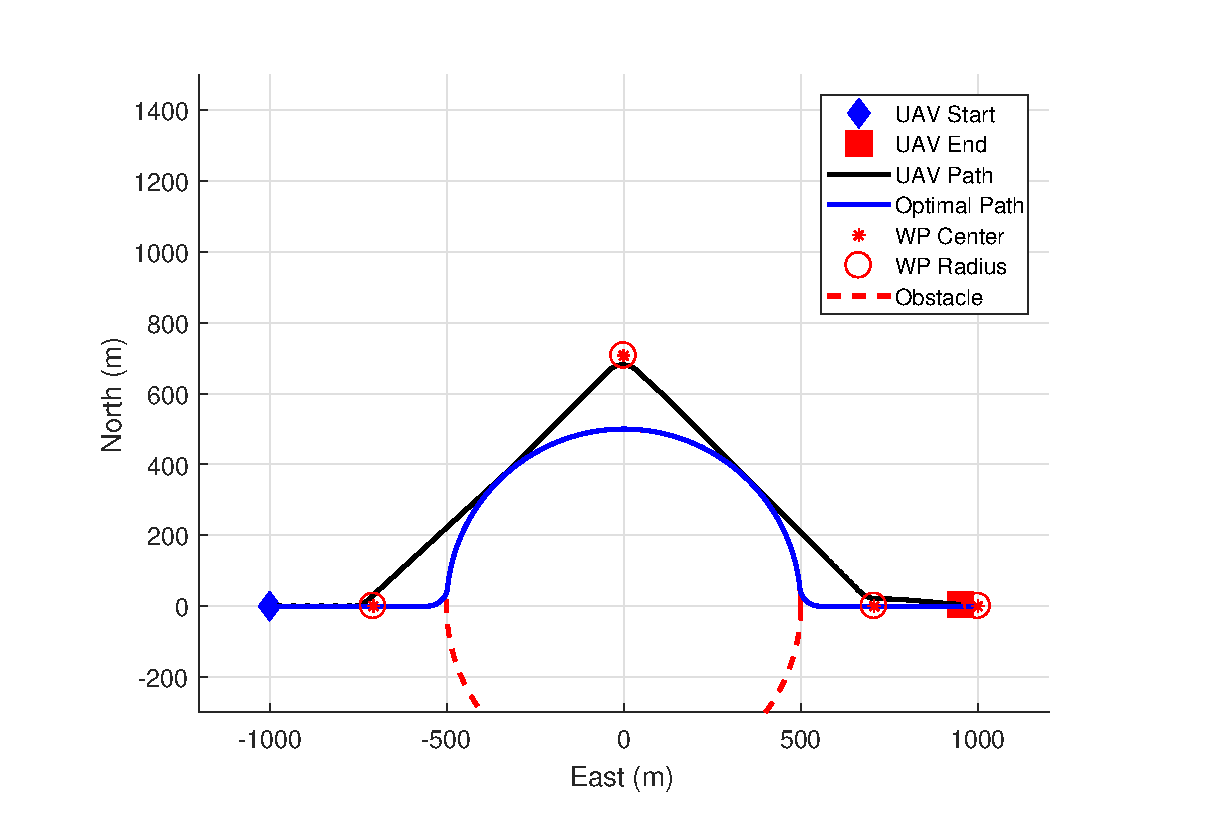
\includegraphics[width=7cm,trim=40 0 60 0,clip] {Figures/Waypoints/1Wpts}}
%		\subfigure []{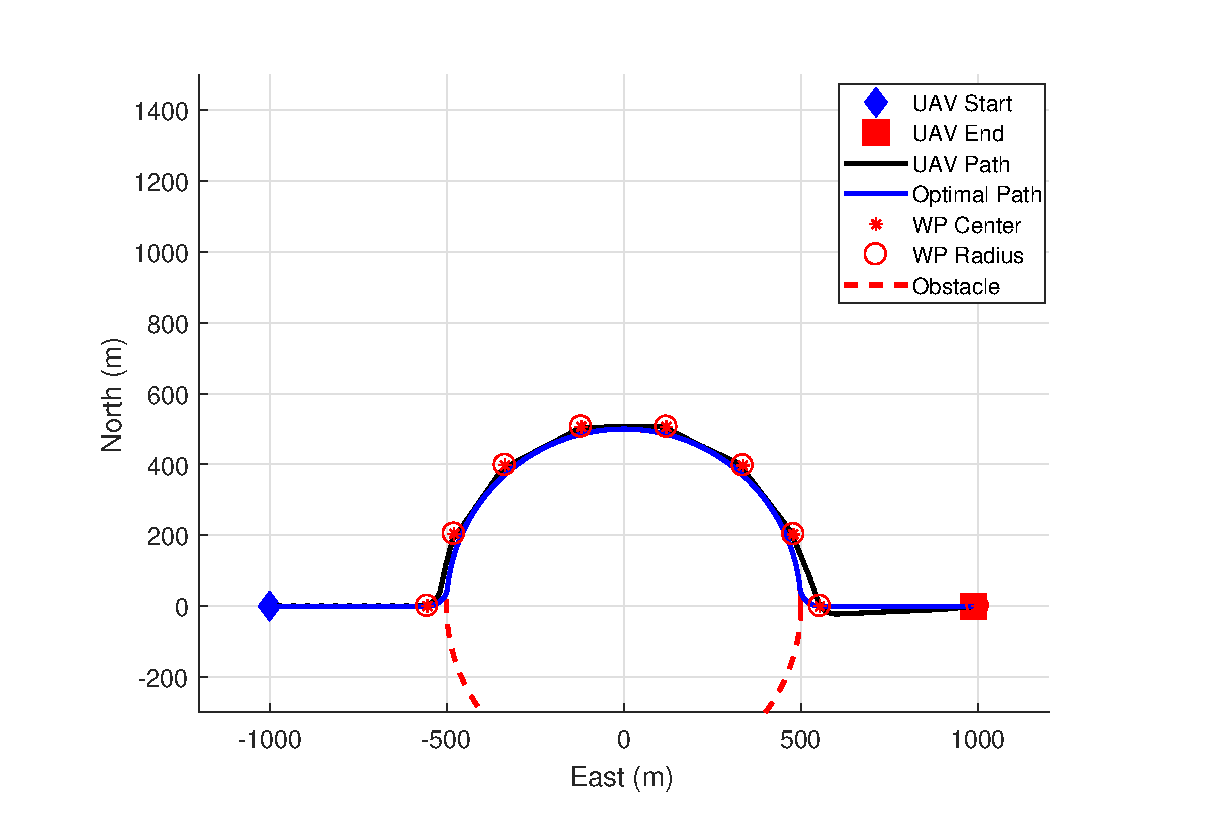
\includegraphics[width=7cm,trim=40 0 60 0,clip] {Figures/Waypoints/6Wpts}}
%		\hspace*{0mm}
%	\end{subfigmatrix}
%	\caption{Obstacle Diversion Waypoints}
%	\label{fig:numWaypointsPath}
%\end{figure}
%
%
%
%\begin{figure}[H]
%	\centering
%	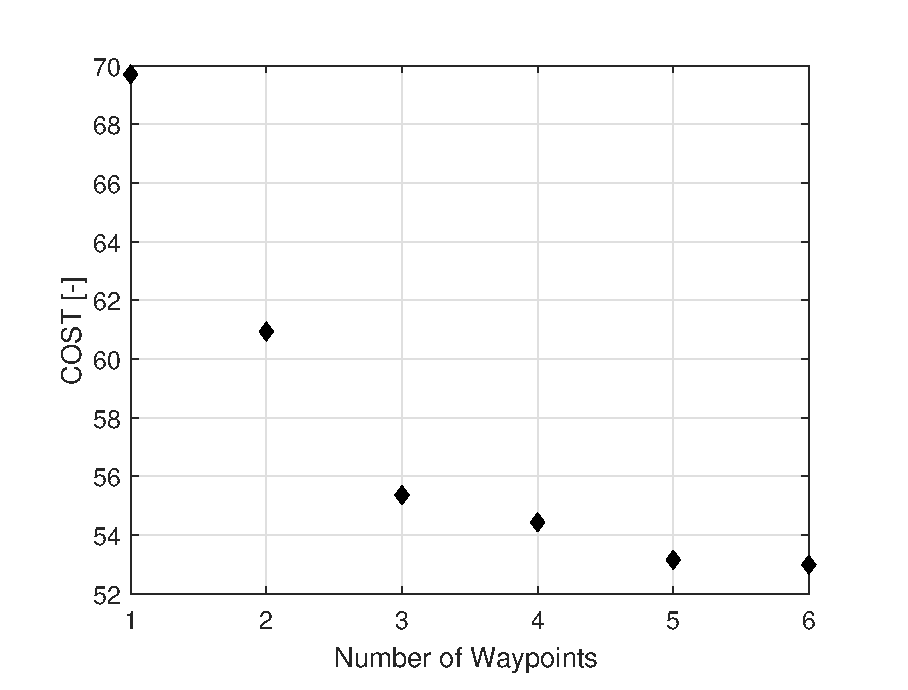
\includegraphics[width=10cm]{Figures/Waypoints/costVnumWpts}
%	\caption{Cost impact versus number of waypoints}
%	\label{fig:numWaypoints}
%\end{figure}




\subsection{Potential Field}


Potential field is based on the principle of artificial attractive and repulsive forces acting on a point mass that is guided to a desired goal while avoiding static and dynamic obstacles \cite{khatib_real-time_1986}. Goal states are represented as an attractive force that pulls a point mass in the direction of minimal energy while obstacles are represented as repulsive forces that act locally to push the point mass away. Potential field is also capable of acting as a path and trajectory planning algorithm \cite{rimon_exact_1992}, possibly eliminating the off-board path planner. 

\begin{figure}[H]
	\centering
	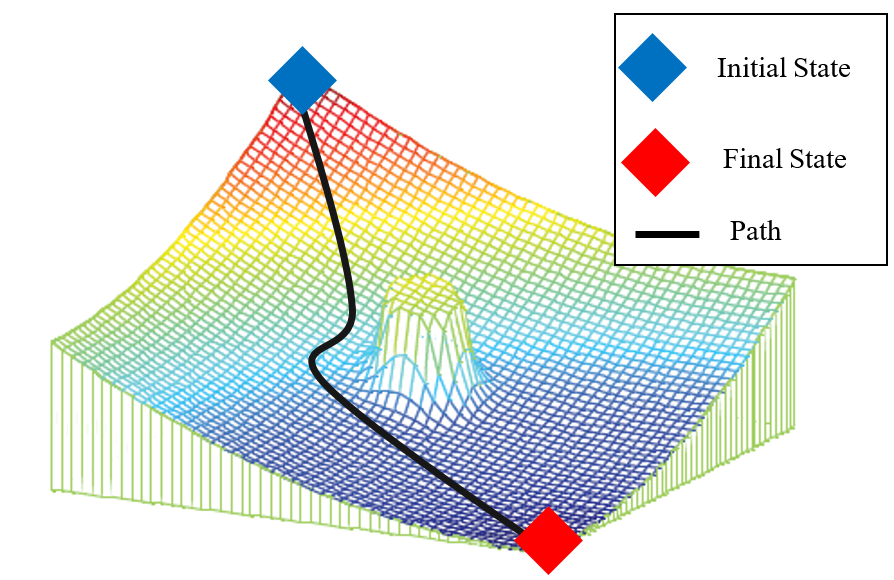
\includegraphics[width=7cm]{PaperFigures/pfObstacle}
	\caption{Single Obstacle Potential Field Gradient \cite{liu_virtual-waypoint_2016}}
	\label{fig:pfobstacle}
\end{figure}


An example of potential field can be found in \cite{borenstein_real-time_1990,borenstein_vector_1991,koren_potential_1991} which allowed for real time goal seeking with obstacle avoidance on a mobile ground robot equipped with ultrasonic sensors. The robot located at $(x_0,y_0)$ is attracted towards a goal with constant magnitude force $\overrightarrow{F_t}$ located at $(x_t,y_t)$ and a distance $d_t$ from the robot. In the immediate area of the robot, an active window exists which records integer certainty values inside discrete cells. Cells containing an obstacle provide a repulsive force $\overrightarrow{F_{i,j}}$ opposite in direction to the line-of-sight from vehicle to cell location $(x_i,y_j)$, where $(i,j$) represents the cell index, $F_{cr}$ is a constant repulsive force, $W$ the vehicle's width, $C_{i,j}$ a cell's certainty, and $d_{i,j}$ the distance to the center of the cell with respect to robots center.

\begin{figure}[H]
	\centering
	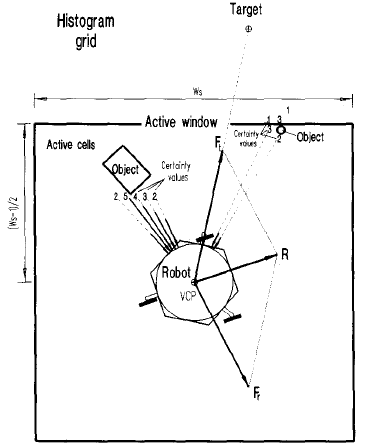
\includegraphics[width=7cm]{PaperFigures/histogram}
	\caption{Virtual force field histogram acting on a mobile robot \cite{borenstein_vector_1991}}
	\label{fig:histogram}
\end{figure}

\begin{equation}\label{eq:vffRepulse}
\overrightarrow{F_{i,j}} = \frac{F_{cr}W^nC_{i,j}}{d^n_{i,j}} \bigg( \frac{x_i-x_0}{d_{i,j}}\hat{x} + \frac{y_i-y_0}{d_{i,j}}\hat{y}\bigg)
\end{equation}

\noindent
The total repulsive force exerted on the robot is determined by summing the active cells, shown in Equation \ref{eq:vffRepulseSum}


\begin{equation}\label{eq:vffRepulseSum}
\overrightarrow{F_r} = \sum_{i,j}\overrightarrow{F_{i,j}}
\end{equation}


\begin{equation}\label{eq:vffGoal}
\overrightarrow{F_t} = F_{ct} \bigg( \frac{x_t-x_0}{d_{t}}\hat{x} + \frac{y_t-y_0}{d_{t}}\hat{y}\bigg)
\end{equation}

\noindent
Summing together attractive and repulsive forces produce a vector $\overrightarrow{R}$ that can be used for heading guidance, shown in Equation \ref{eq:vffHeading}.

\begin{equation}\label{eq:vffHeading}
\overrightarrow{R} = \overrightarrow{F_r} + \overrightarrow{F_t}
\end{equation}

Major drawbacks to potential field were identified in \cite{koren_potential_1991} consisting of local minimum and oscillations in corridors. The local minimum problem occurs when closely spaced obstacle's potential combine to produce a well on the descent gradient where a pre-mature stable point is reached, shown in Figure \ref{fig:pfLocalMin}. Additionally, closely spaced obstacles may also be difficult to pass between, shown in Figure \ref{fig:vff}a. Oscillations can also be experienced near obstacles or in narrow passages at high speeds, shown in Figure \ref{fig:vff}b.



 

\begin{figure}[H]
	\begin{subfigmatrix}{2}% number of columns
		\centering
		\subfigure []{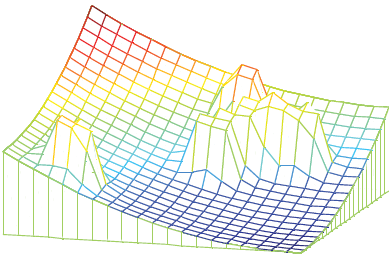
\includegraphics[width=7cm] {PaperFigures/pfObstacleLocalMin}}
		\subfigure []{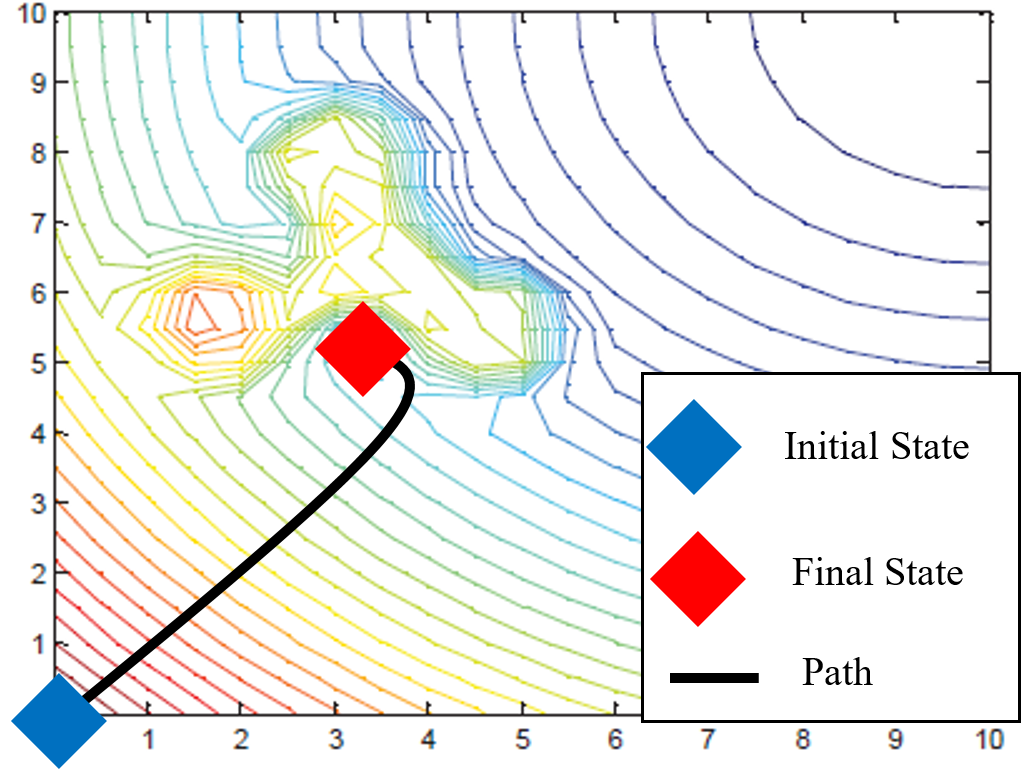
\includegraphics[width=7cm] {PaperFigures/pfObstacleLocalMinTopology}}
	\end{subfigmatrix}
	\caption{Potential Field Local Minimum \cite{liu_virtual-waypoint_2016}}
	\label{fig:pfLocalMin}
\end{figure}

Proposed solutions to local minimum include object clustering and virtual waypoint method \cite{liu_virtual-waypoint_2016}, virtual escaping route \cite{kim_escaping_2009}, and use of navigation functions \cite{goerzen_survey_2010}. Oscillations in potential field were addressed in \cite{lei_tang_novel_2010} and \cite{li_efficient_2012}.

\begin{figure}[H]
	\begin{subfigmatrix}{2}% number of columns
		\centering
		\subfigure []{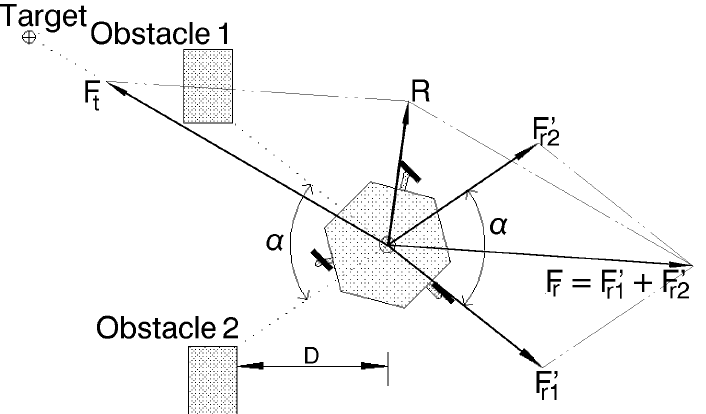
\includegraphics[width=9cm] {PaperFigures/multipleObsVff}}
		\subfigure []{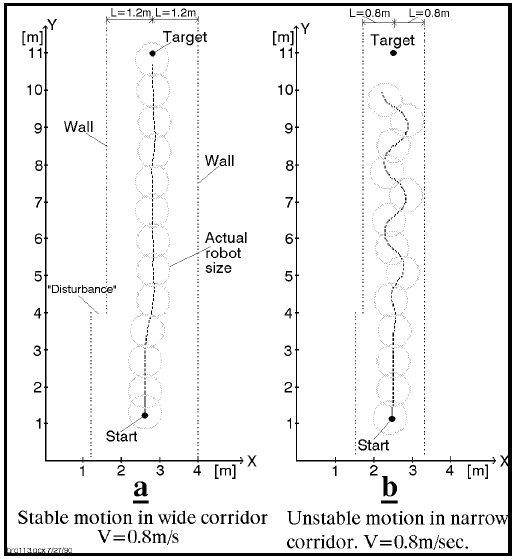
\includegraphics[width=6cm] {PaperFigures/unstableCooridorMotionVff}}
	\end{subfigmatrix}
	\caption{Potential Field Local Minimum \cite{liu_virtual-waypoint_2016}}
	\label{fig:vff}
\end{figure}

Navigation functions \cite{goerzen_survey_2010} and obstacle clustering \cite{liu_virtual-waypoint_2016} have been used to prevent local minimums in potential field. Navigation functions relate kinematic constraints to the gradient potential to produce a bounded and local minimum free solution \cite{rimon_exact_1992}. Clustering closely spaced obstacles into a single and equally repulsive obstacle prevents local minimum from forming, shown in Figure \ref{fig:obstacleclustering}.  

\begin{figure}[H]
	\centering
	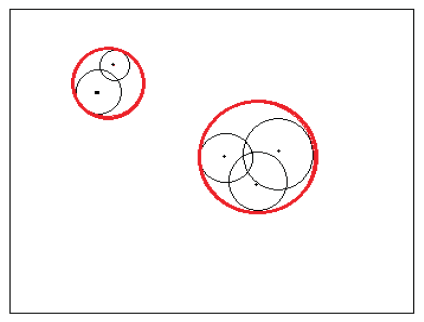
\includegraphics[width=6cm]{PaperFigures/obstacleClustering}
	\caption{Obstacle Clustering \cite{liu_virtual-waypoint_2016}}
	\label{fig:obstacleclustering}
\end{figure}

Potential Field's ability to avoid obstacles and combine path planning, trajectory planning, and control into a single computationally inexpensive system makes it an attractive motion control system for robots seeking a singular point, even with the limitations discussed in \cite{koren_potential_1991}. \\

In addition to local minimum and oscillations, potential field may not be ideal for providing guidance to return to a sensor path after avoiding an obstacle. Unlike the mobile ground robots in \cite{borenstein_real-time_1990}, fixed wing UAVs must maintain a minimum forward velocity, have limited turning radius, and cannot converge to a single point. Vehicles with velocity and turn rate constraints may not return to a pre-planned path once the obstacle has been avoided, shown in Figure \ref{fig:vffSimulated}. Vector fields that direct a UAV to paths connecting waypoints have been developed using Lyapunov and gradient vector field techniques. 


\begin{figure}[H]
	\centering
	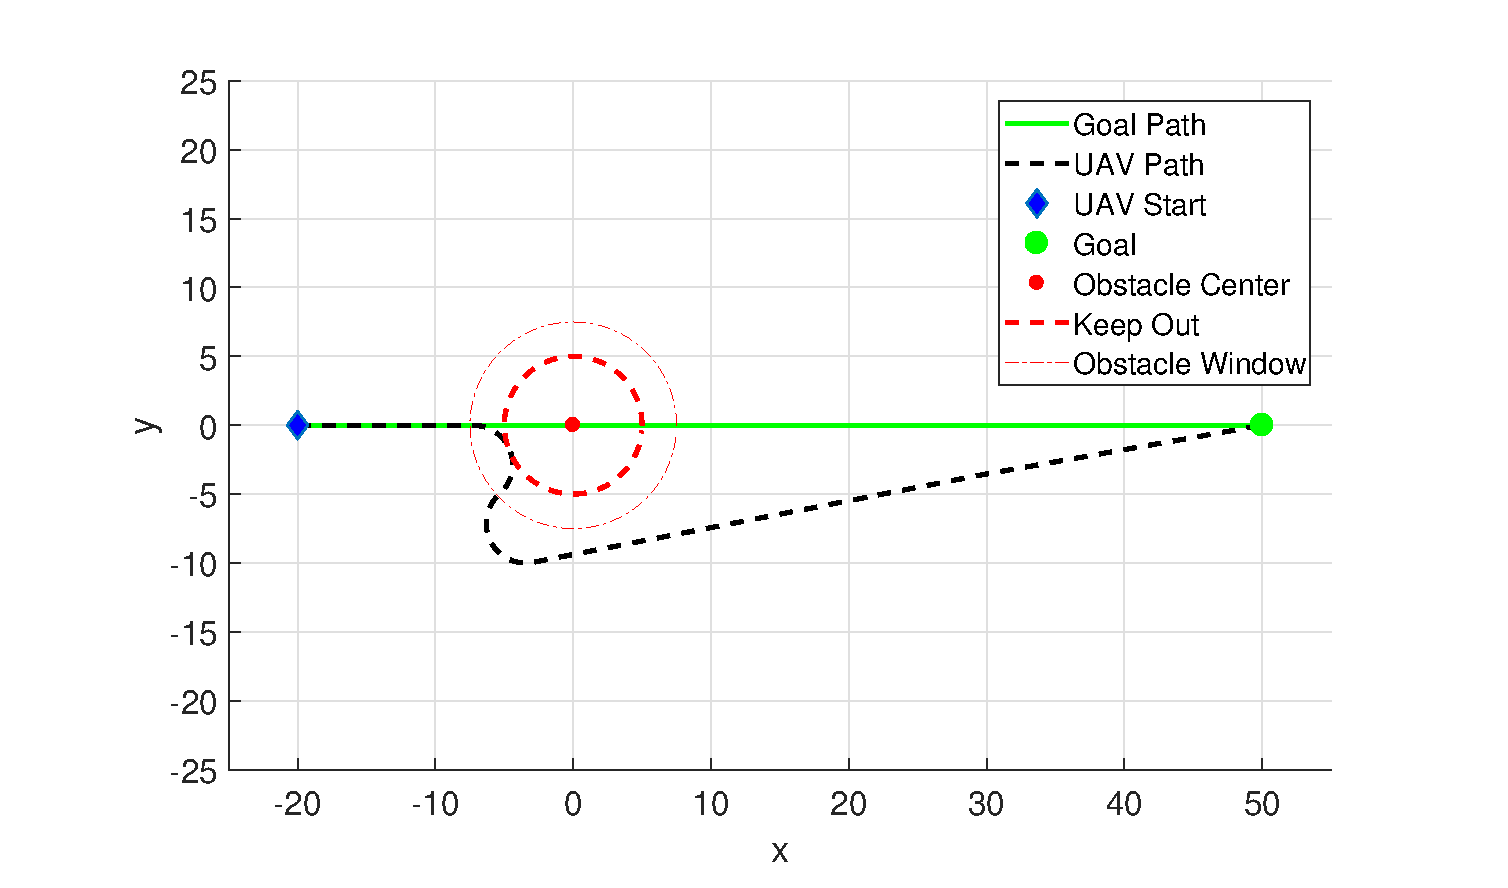
\includegraphics[width=15cm]{PaperFigures/Literature/vffSimulated}
	\caption{UAV avoiding obstacle with VFF Guidance}
	\label{fig:vffSimulated}
\end{figure}


%\subsection{\hl{Path Following Vector Field Guidance}}
%
%Path following can be accomplished with vector fields which produce a heading guidance that asymptotically converges and circulates a path. A comparison between vector field and waypoint guidance techniques was presented in \cite{sujit_unmanned_2014} where each method was evaluated based on its complexity, robustness, and accuracy. Vector field produced guidance that was both robust to external wind disturbances while maintaining a low cross track error.
%
%
%The UAV guidance system is responsible for taking high level pre-planned paths from the ground station and providing a reference heading command to the control system. Several methods for path following guidance were investigated in \cite{sujit_unmanned_2014} consisting of carrot chasing \cite{manjunath_application_2016}, non-linear guidance law, pure line-of-sight \cite{fortuna_cascaded_2015}, linear quadratic regulator \cite{capello_simulation-based_2012}, and vector field method \cite{nelson_cooperative_2005}. A Monte Carlo simulation with wind disturbances was conducted for the guidance methods above in \cite{sujit_unmanned_2014} to determine each method's performance based on accuracy, robustness, and control effort. The vector field method followed the path with the least tracking error and control effort which is the primary goal of path following. 


%\section{Vector Field Guidance}
%\subsection{Introduction to Vector Field Guidance}
% \hl{Vector Field is a guidance and control approach that can be used to transition a robotic system from an initial state to a final state. Final states, or goals, act as artificial attractive forces that pull on the robotic system while obstacles act as artificial repulsive forces that push the robotic system away. Classes of vector fields can be categorized as point seeking or path following algorithms. Potential Field and Virtual Force Field (VFF) methods converge to a single point and avoid obstacles by applying artificial attractive and repulsive forces. Lyapunov and Gradient Vector Fields provide guidance that asymptotically converges and follows a path. Obstacle avoidance has been achieved with Gradient Vector Fields by assigning repulsive weights to a convergence term. Weights currently act as a high level specification of the desired guidance behavior and may be further optimized.} 

\subsection{Lyapunov Vector Fields}



Lyapunov vector fields for converging and following straight and circular paths were described in \cite{nelson_cooperative_2005}. For converging and following a straight path, a guidance vector $\chi^{d}$ is determined in Equation \ref{eq:lyapunovStraight}, where $\chi^{\infty}$ is the course approach angle, $y$ is the lateral distance to the path, and $k$ is a positive constant that determines the rate of transition between convergence and following. An example of a Lyapunov vector field converging and following a straight line is shown in Figure \ref{fig:vfPathPrimitives}a.



% and are defined in Equations \ref{eq:lyapunovStraight} and \ref{eq:lyapunovCirc} respectively.

%------ Nelson VF equations -----
\begin{equation}\label{eq:lyapunovStraight}
\chi^d(y) = -\chi^{\infty}\frac{2}{\pi}\tan^{-1}(ky)
\end{equation}



For converging and following a circular path, a guidance vector $\chi^{d}$ is determined in Equation \ref{eq:lyapunovCirc}, where $\gamma$ is the UAVs angular position with respect to the circle, $r$ is the paths radius, $d$ is the distance from the circles center, and $k$ is a positive constant that determines the transition behavior. An example of a Lyapunov vector field for converging and following a circular path is shown in Figure \ref{fig:vfPathPrimitives}b.

\begin{equation}\label{eq:lyapunovCirc}
\chi^d(d) = \gamma-\frac{\pi}{2}-\tan^{-1} \bigg(k \frac{d-r}{r} \bigg)
\end{equation}


\begin{figure}
	\centering
	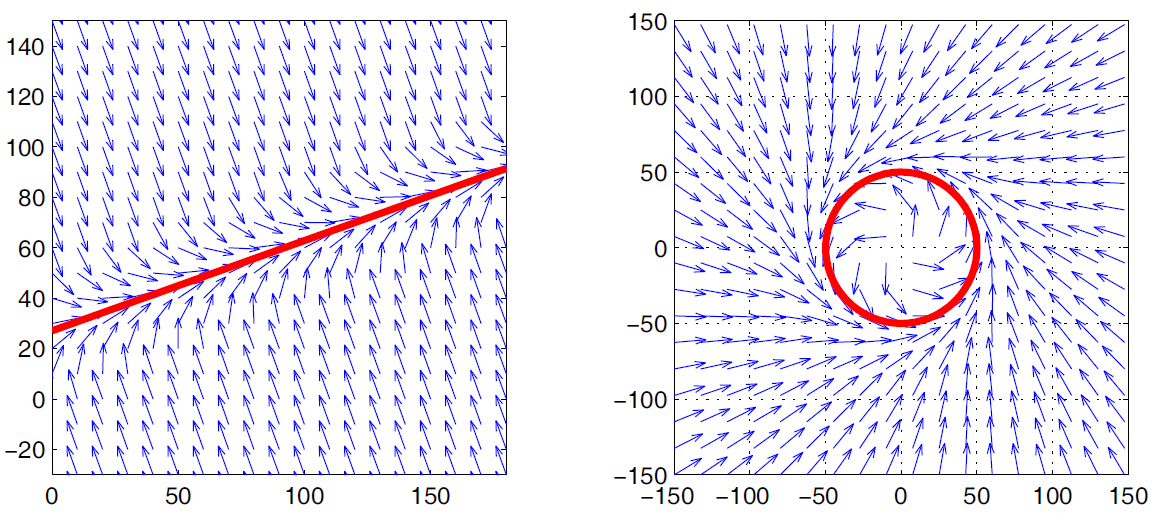
\includegraphics[width=13cm]{PaperFigures/nelsonLyapunov}
	\caption{Lyapunov vector field for straight line and circular primitives \cite{nelson_cooperative_2005}}
	\label{fig:vfPathPrimitives}
\end{figure}




%A circular Lyapunov vector field can be generated by the methodology described in \cite{frew_cooperative_2007}. Given the Lyapunov function:
%
%
%$y$ lateral distance from path \\
%$\chi$ difference between direction of path and course of UAV \\
%$k$ positive constant that influences the rate of transition \\
%$\chi^{\infty}$  course approach angle at large distance \\
%$\chi^{d}$ is commanded heading \\
%
%$d$ radial distance UAV from center of orbit \\
%$\gamma$ angular position with respect to orbit center \\
%$r$ orbit radius \\
%
%
%
%
%\begin{figure}[H]
%	\begin{subfigmatrix}{2}% number of columns
%		\centering	
%		\subfigure []{\includegraphics[width=7.5cm] {Figures/lineConvcirc}}
%		\subfigure []{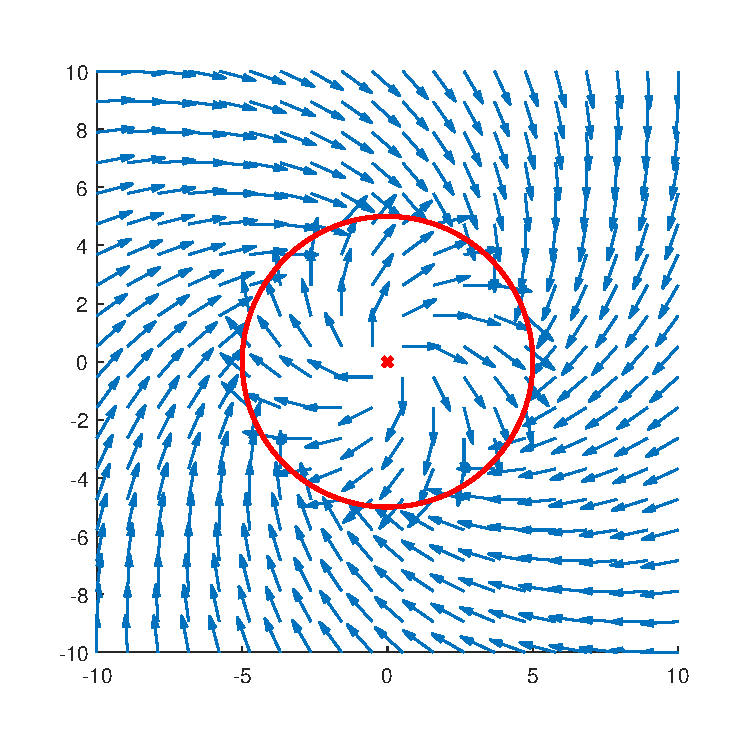
\includegraphics[width=7.5cm] {Figures/circConvCirc}}
%		\hspace*{0mm}
%	\end{subfigmatrix}
%	\caption{Vector field converging and following a) straight path b) circular path}
%	\label{fig:vfPrimitives}
%\end{figure}
%
%
%\begin{equation}\label{eq:lyapunovfunction}
%V(x,y) = (r^2 - r_d^2)^2
%\end{equation}
%where $r$ is given by the equation
%\begin{equation}
%r = \sqrt{x^2+y^2}
%\end{equation}
%and the total time derivative of Equation \ref{eq:lyapunovfunction} is
%\begin{equation}\label{eq:totaltimederivative}
%\dot{V}(x,y) = \nabla{V} \cdotp [\dot{x},\dot{y}]^{T}
%\end{equation}
%Utilizing the following equation to select the desired relative velocity $\dot{x}$ and $\dot{y}$
%\begin{equation}
%\overrightarrow{V}_{Lyapunov}\!=\!\begin{bmatrix} \dot{x_d} \\ \dot{y_d} \end{bmatrix}\!= \alpha\!\left(\dfrac{-v}{r}\right)\!\begin{bmatrix} x \dfrac{r^2-r_d^2}{r^2+r_d^2} + y \dfrac{2 r r_d}{r^2+r_d^2} \\[12pt] y \dfrac{r^2-r_d^2}{r^2+r_d^2} - x \dfrac{2 r r_d}{r^2+r_d^2} \end{bmatrix}
%\end{equation}
%and assuming $\alpha$\,=\,1 and $r$\,=\,1, the final Lyapunov VF equation is generated:
%\begin{equation}\label{eq:lyapunovvf}
%\overrightarrow{V}_{Lyapunov} = \frac{v}{r^2+r_d^2} \begin{bmatrix} - x (r^2-r_d^2) - y (2 r r_d) \\[6pt] - y (r^2-r_d^2) + x (2 r r_d) \end{bmatrix}
%\end{equation}



%Straight and circular path vector fields can be selectively activated throughout flight to form more complex paths, shown in \cite{nelson_cooperative_2005,nelson_vector_2006,nelson_vector_2007,jung_unmanned_2016}. Lyapunov vector field for curved path following was presented in \cite{griffiths_vector_2006} which may allow for more complex paths and eliminates the need to switch between vector fields. \\


%
%==========================\\
%Lyapunov vector fields produce heading guidance that asymptotically converges and circulates along a path passing through waypoints. Paths can be built from straight line and circular arc primitives taking UAV kinematic constraints into consideration. Vector Fields that guide to straight line and circular paths was introduced in \cite{nelson_cooperative_2005}. Farther away from the path, vectors are constant and point in the direction perpendicular to the path. Within a transition region the vectors begin to rotate and point more parallel to the path. Vectors on the path point directly in the direction of the path. Lyapunov vector fields for straight line and circular arcs are shown in Figure \ref{fig:nelsonlyapunov}.
%
%=====================================

Straight and circular path vector fields can be selectively activated throughout flight to form more complex paths, shown in \cite{nelson_cooperative_2005,nelson_vector_2006,nelson_vector_2007,jung_unmanned_2016} and Figure \ref{fig:urbanfollowingnelson}. Each path primitive has a vector field associated with it and determining which field to use can be approached in two different ways. Fields from all of the primitives can be summed together similar to the attractive and repulsive forces in potential field. Second, fields can be selectively activated and deactivated based on the position of the UAV. Summing together vector fields, as pointed out in \cite{nelson_cooperative_2005}, can result in several problems including dead zones, sinks, and singularities. Selectively activating each vector field as a UAV nears waypoints was used in \cite{nelson_cooperative_2005,nelson_vector_2006,nelson_vector_2007,jung_unmanned_2016}.

\begin{figure}[H]
	\centering
	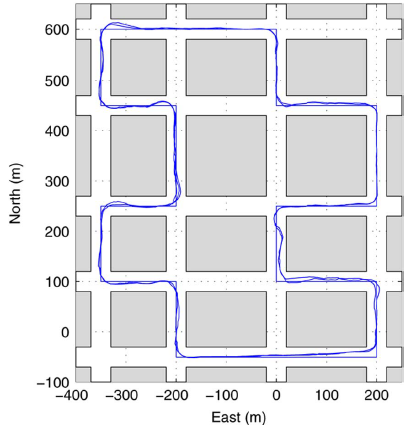
\includegraphics[width=7cm]{PaperFigures/urbanFollowingNelson}
	\caption{Straight path following in urban environment \cite{nelson_cooperative_2005} using Lyapunov Vector Field}
	\label{fig:urbanfollowingnelson}
\end{figure}

Lyapunov Vector field construction for curved paths was presented in \cite{griffiths_vector_2006} and is shown in Figure \ref{fig:griffiths}. Constructing a Vector Field for an arbitrary curve may allow for more complex paths and could eliminate the need for switching between primitives. 

\begin{figure}[H]
	\centering
	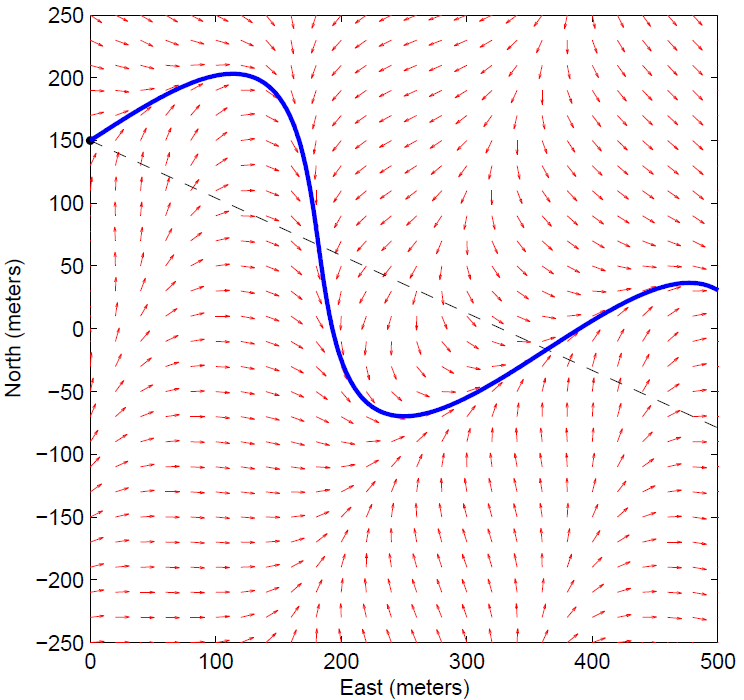
\includegraphics[width=7cm]{PaperFigures/griffiths}
	\caption{Lyapunov vector field approach curved path asymptotically \cite{griffiths_vector_2006}}
	\label{fig:griffiths}
\end{figure}


Primitive circular vector fields were modified in \cite{frew_lyapunov_nodate,frew_cooperative_2007} via non-linear coordinate transformations to produce elliptical \ref{fig:lyapunovFrew}a, or racetrack \ref{fig:lyapunovFrew}b, fields. Transforming the circular field as a function of a Kalman filter's covariance matrix when sensing an uncertain target was investigated in \cite{frew_cooperative_2007}. 

\begin{figure}[h]
	\begin{subfigmatrix}{2}% number of columns
		\centering
		\subfigure []{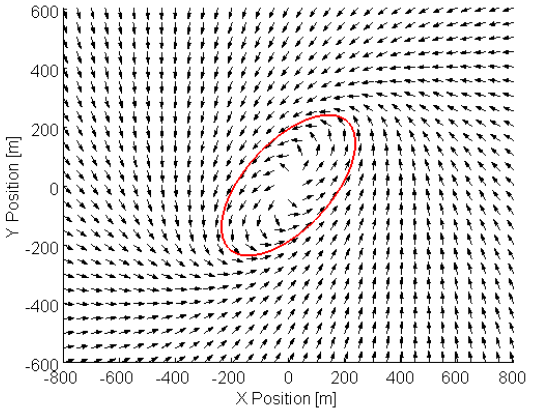
\includegraphics[width=8cm] {PaperFigures/lyapunovFrewUncertain}}
		\subfigure []{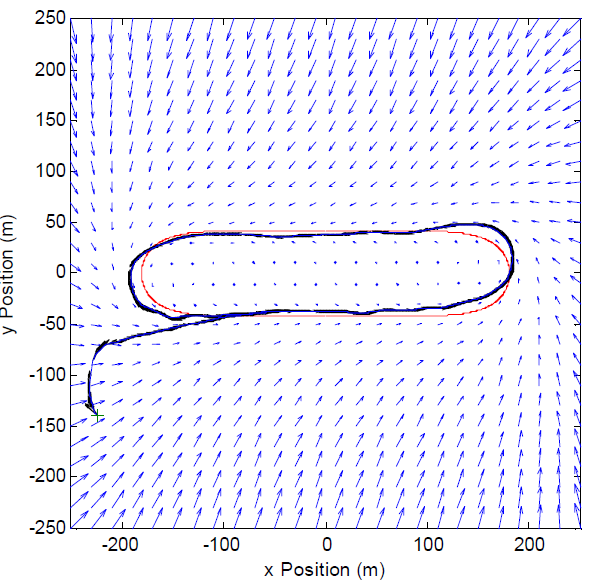
\includegraphics[width=6.25cm] {PaperFigures/lyapunovFrew}}
		%		\hspace*{1cm}
	\end{subfigmatrix}
	\caption{Elliptical VF produced by non-linear coordinate transformations a)\cite{frew_cooperative_2007} and b) \cite{frew_lyapunov_nodate}}
	\label{fig:lyapunovFrew}
\end{figure}

Target tracking Tangent Plus Lyapunov Vector Field (TPLVF) was introduced in \cite{chen_tracking_2009} that produced shorter paths compared to Lyapunov alone. Outside of the standoff circle, tangent vectors provided the shortest distance to a standoff circle. Inside the standoff circle, no tangent lines exist and Lyapunov was used in its place. Figure \ref{fig:lyapunovChen} shows the difference in paths taken for Lyapunov and tangent vector fields outside the standoff circle. The TPLVF was later used for path planning to avoid obstacles in \cite{chen_uav_2013} while \cite{liang_tangent_2017} constructed a tangent vector field for curved paths.

\begin{figure}
	\centering
	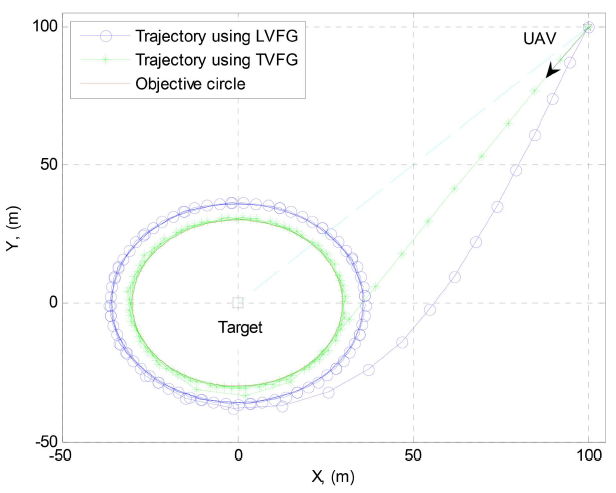
\includegraphics[width=10cm]{PaperFigures/lyapunovChen}
	\caption{Tangent plus lyapunov vector fields for shortest path target tracking \cite{chen_uav_2013}}
	\label{fig:lyapunovChen}
\end{figure}


\subsection{Path Planning Vector Fields}
All methods that consider obstacles thus far built a vector field that guides the UAV to an obstacle free path. Another approach is to use vector fields as a high level specification for heuristic path planning algorithms \cite{pereira_framework_2016}. An optimal Rapid Random Trees (RRT*) algorithm used a vector field as a guide to explore the configuration space of the UAV for an obstacle free path. Branches extend from the root, or initial location of the UAV, randomly throughout the map with a finite deviation from the initial vector field. When a branch encounters an obstacle it is trimmed and no longer explored. The path of minimum cost, or least distance, is selected for the UAV to use as a reference path. An example of the algorithm is shown in Figure \ref{fig:rrtvf}.

\begin{figure}[H]
	\centering
	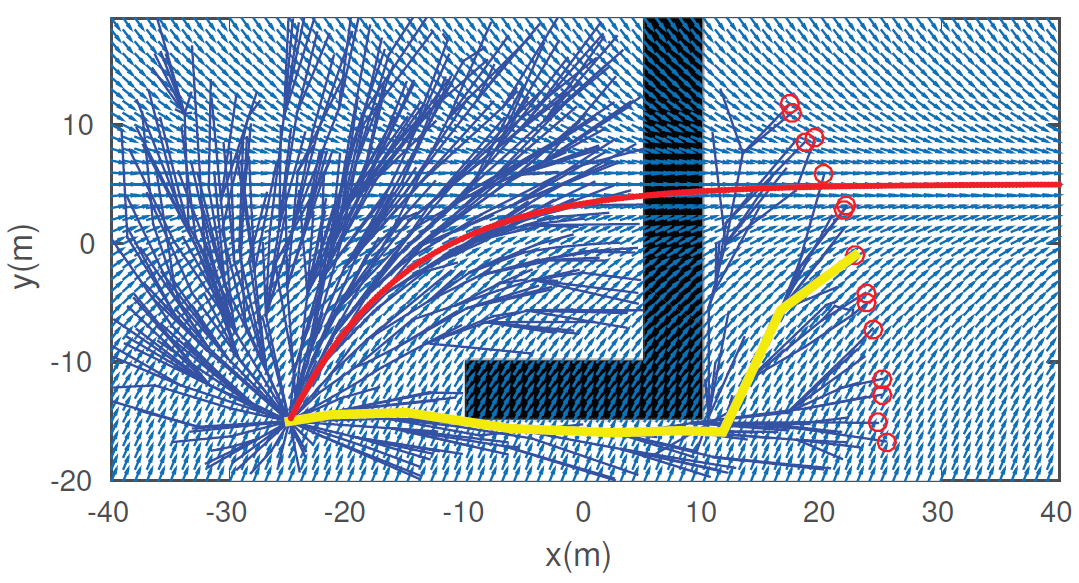
\includegraphics[width=12cm]{PaperFigures/rrtVF}
	\caption{RRT* path planner with a VF used as a task specification \cite{pereira_framework_2016}}
	\label{fig:rrtvf}
\end{figure}


A Vector Field was constructed inside a configuration space with edges defined by Delauny triangulation (DT) in \cite{pimenta_fully_2007}.  A simulation of a robot traversing a vector field inside a set of DTs can be seen in Figure \ref{fig:cdtVF}. Vector fields designed to stay inside a region of DTs may be used with optimal path planning algorithms for navigating urban environments \cite{md_simplex_2017}.


\begin{figure}
	\centering
	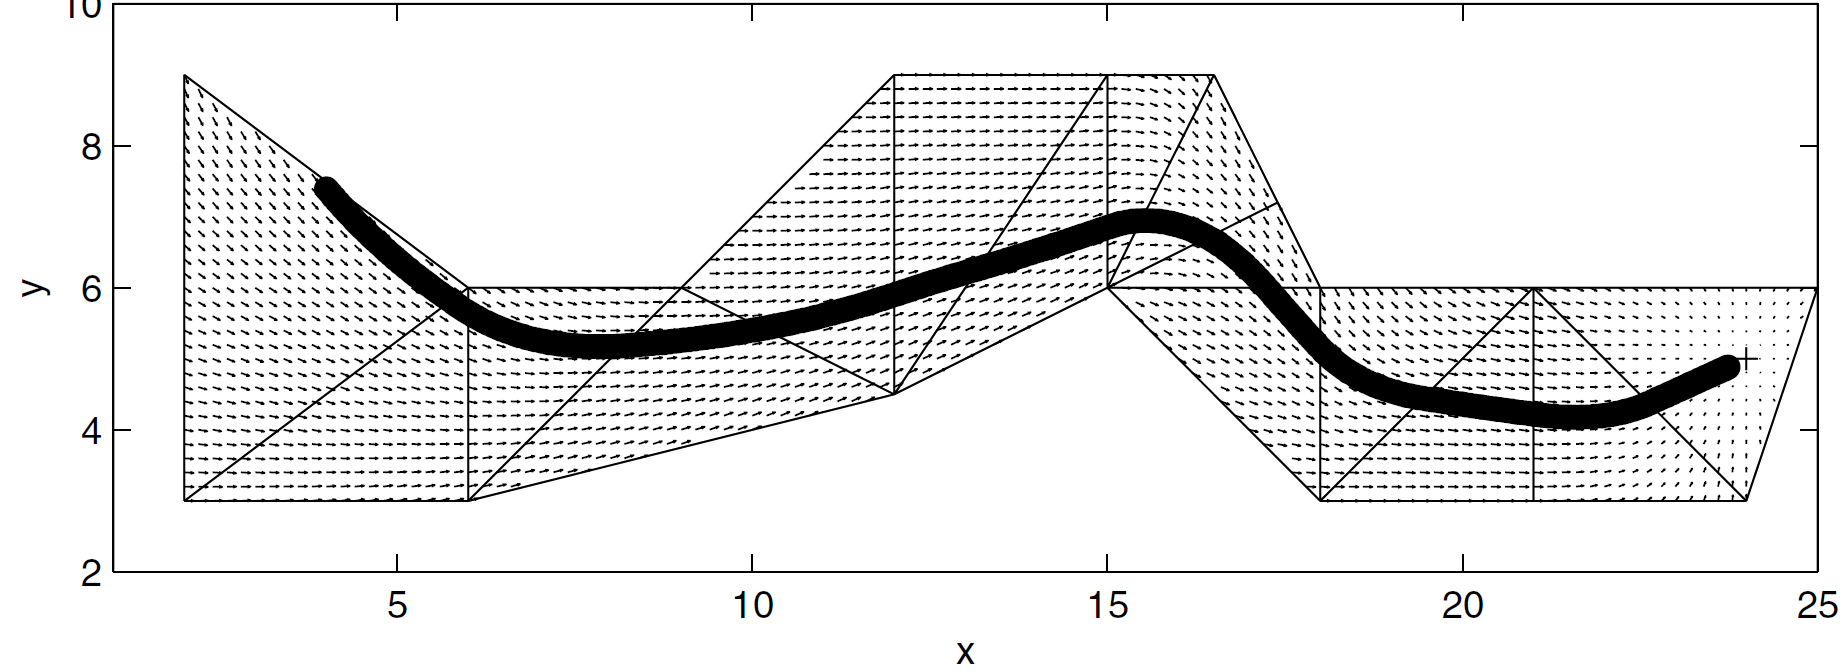
\includegraphics[width=15cm]{PaperFigures/cdtVF}
	\caption{Vector field within a set of delaunay triangles \cite{pimenta_fully_2007}}
	\label{fig:cdtVF}
\end{figure}

So far all of the vector field methods discussed have avoided obstacles by planning paths around them. Paths are typically calculated at the ground station and if communication is lost a new path may not be relayed to a UAV encountering a new obstacle. A possible solution is using vector fields to provide a repulsive force such as that seen in \cite{panagou_motion_2014,zhou_vector_2014} [wwc]. 

\subsection{Gradient Vector Field}
The Gradient Vector Field (GVF) method produces a similar field to LVF, however has several advantages over LVFs. GVF produces an \textit{n}-dimensional vector field that converges and circulates to both static and time varying paths \cite{goncalves_artificial_2009}. Additionally, convergence, circulation, and time-varying terms that make up the GVF are decoupled from each other allowing for easy weighting of the total field \cite{goncalves_circulation_2010}. GVFs converge and circulate at the intersection, or level set, of $n-1$ dimensional implicit surfaces ($\alpha_i:\mathbb{R}^n\rightarrow\mathbb{R} | i=1,...,n-1$). The integral lines of the field are guaranteed to converge and circulate the level set when two conditions are met: $1)$ the implicit surface functions are positive definite and $2)$ have bounded derivatives. Consider the space with dimensions in set \textbf{q}:

%The Goncalves Vector Field (GVF) method for producing vector fields has several advantages over the Lyapunov vector field generation methods.


\begin{equation}
\mathbf{q} = \begin{bmatrix} x_1, x_2, ..., x_{n}\end{bmatrix}
\end{equation}

\noindent
The total vector field $\overrightarrow{V}$ is calculated by:
\begin{equation}\label{eq:GVF}
\overrightarrow{V} = G \nabla V + H \wedge_{i=1}^{n-1}\nabla_q\alpha_i  - LM(\alpha)^{-1} a(\alpha)
\end{equation}

\noindent
or in component form:

\begin{equation}\label{simpleGVF}
\overrightarrow{V} = \overrightarrow{V}_{conv} + \overrightarrow{V}_{circ} + \overrightarrow{V}_{tv} 
\end{equation}	

\noindent
where $\overrightarrow{V}_{conv}$ produces vectors perpendicular to the path, $\overrightarrow{V}_{circ}$ produces vectors parallel to the path, and $\overrightarrow{V}_{tv}$ is a feed-forward term that produces vectors accounting for a time varying path. The scalars $G$,$H$, and $L$ weight convergence, circulation, and time varying components respectively. 

\noindent
Convergence is calculated by:

\begin{equation}
% Total field with Conv, Circ, and Time
\overrightarrow{V}_{conv} = G \nabla V  
\label{convOnly}
\end{equation}

\noindent
where scalar $G$ is multiplied by the gradient of the definite potential function $V$:

\begin{equation}
V = -\sqrt{{\alpha_1}^2 + {\alpha_2}^2}
\end{equation}


\noindent
Circulation is calculated by taking the wedge product of the gradient:

\begin{equation}
% Total field with Conv, Circ, and Time
\overrightarrow{V}_{circ} =  \wedge_{i=1}^{n-1}\nabla_q\alpha_i 
\label{circOnly}
\end{equation}

\noindent
In the case of $(n=3)$ the wedge product simplifies as the cross product:

\begin{equation}
% Total field with Conv, Circ, and Time
\overrightarrow{V}_{circ} =  \nabla_q\alpha_1 \times \nabla_q\alpha_2 
\label{circOnlySimp}
\end{equation}

\noindent
The feed-forward time-varying component is calculated by:
\begin{equation}
\label{tv}
\overrightarrow{V}_{tv} = M^{-1}a
\end{equation}

\noindent
where,

\begin{equation}
\label{mMatrix}
M =\begin{bmatrix}
\nabla\alpha_1^T \\
\nabla\alpha_2^T \\
(\nabla\alpha_1 \times \nabla\alpha_2)^T
\end{bmatrix}
\end{equation}

\begin{equation}
\label{aVector}
a =\begin{bmatrix}
\frac{\partial \alpha_1}{\partial t} \quad   \frac{\partial \alpha_2}{\partial t} \quad   0
\end{bmatrix}^T
\end{equation}


In \cite{goncalves_artificial_2009,goncalves_circulation_2010,goncalves_vector_2010} GVFs $h$ were constructed to control the velocity $\dot{q}$ of holonomic robots by $\dot{q}=h$. Constant speed  $u$ was controlled by calculating the weighting scalars $G$,$H$, and $L$ that maintained the condition $||\dot{q}|| = u$. Other studies normalized the vector $\overrightarrow{V}$ and used it as a heading guidance while assuming velocity is held constant by the autopilot \cite{gerlach_autonomous_2014,wwc}. Assuming velocity is controlled by a separate system frees up the vector field scalars to modify field behavior for other applications, such as obstacle avoidance. 
 
 
 The standoff tracking and avoidance scenario presented in \cite{wwc} used GVF as a heading guidance and static GVF weights to specify high level guidance behavior. A fixed UAV was tasked with loitering around a slow moving ground target while avoiding obstacles. A circular attractive time-varying vector field $\overrightarrow{V}_{path}$ was attached to a moving ground target and summed with repulsive obstacle vector fields $\overrightarrow{V}_{o}$ centered at the obstacles to provide the guidance $\overrightarrow{V}$ in Equation \ref{summedAttRepulsive}. 
 
 
 \begin{equation}
 \overrightarrow{V} = \overrightarrow{V}_{attractive}+P\overrightarrow{V}_{repulsive}
 \label{summedAttRepulsive}
 \end{equation}
 
 \noindent
 The strength of repulsive obstacle fields were weighted by the hyperbolic tangent decay function $P(d)$ in Equation \ref{repulsiveDecay}, where $d$ is the range to the obstacle and $R$ is the radius of the decay
 
 \begin{equation}
 P = R\frac{tanh(2\pi d-\pi)+1}{2}
 \label{repulsiveDecay}
 \end{equation}
 
 \noindent
 The performance of LVF [21] and GVF \cite{goncalves_artificial_2009,goncalves_circulation_2010,goncalves_vector_2010} were compared for their cross track error with respect to the loiter circle in [wwc]. GVF had favorable performance due to compensation for a time-varying vector field. The path of the fixed wing UAV tracking a slow moving ground target while avoiding static obstacles is shown in Figure \ref{fig:gvfMovingTarget}


\begin{figure}[H]
	\centering
	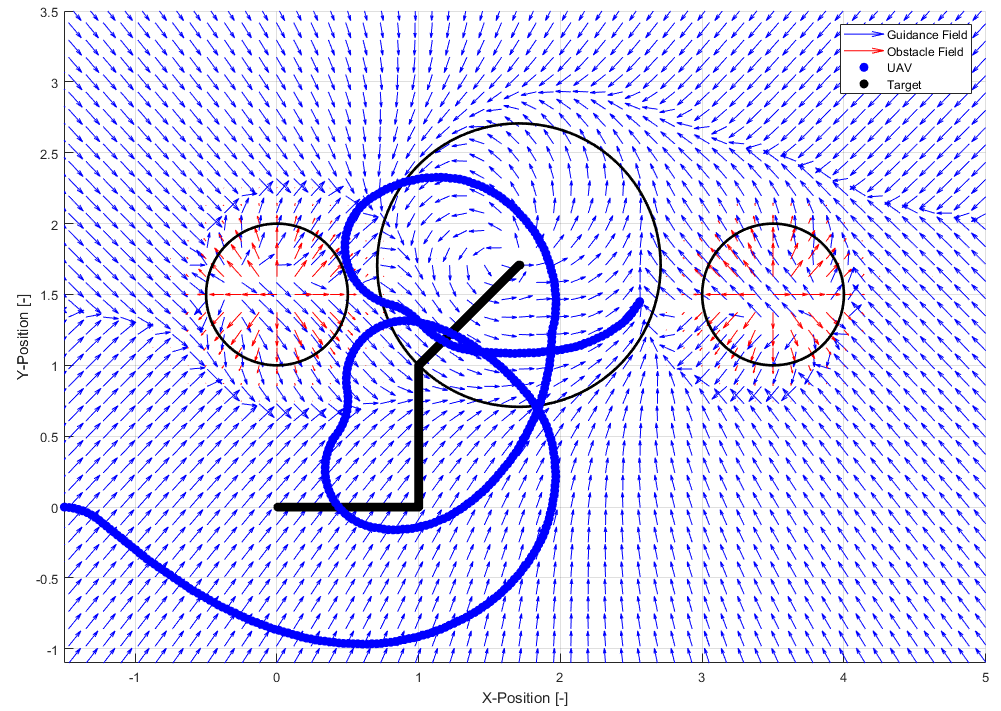
\includegraphics[width=10cm]{PaperFigures/gvfMovingTarget}
	\caption{Place holder image of UAV following ground target \cite{wwc}}
	\label{fig:gvfMovingTarget}
\end{figure}

Summing attractive and repulsive vector fields may result in null guidance where the fields cancel, providing no guidance. The presence of singularities were not addressed in \cite{wwc}, mentioned briefly in \cite{nelson_cooperative_2005} and observed in \cite{panagou_motion_2014}. For fixed wing UAVs the lack of guidance may prevent the UAV from avoiding an obstacle, while multi-rotor UAVs may end up in a trap situation. Singularities may be present at any location where a goal field and obstacle field are of equal strength. Detecting singularities and modifying the GVF for an improved obstacle avoidance is the contribution of this research.



%The GVF weights are decoupled from each term calculation, therefore modifications to the GVF weights do not require a new derivation of the resulting field. Magnitude of the weights effectively scales the contribution of each term. Negating the GVF weights has been used to provide a repulsive field for obstacle avoidance in \cite{wwc} for a UAV tracking a moving loiter circle. Assigning weights \textbf{G=-1} and \textbf{H=L=0} rotates the attractive field vectors in Figure \ref{fig:gvfCircAttractive}b 180$^\circ$ about the tail of each vector, which is shown in Figure \ref{fig:gvfRepulsiveRadius}a. Note how the repulsive field vectors point away from the circular curve for the entire configuration space. Encircling an obstacle by a path produces vectors that may provide guidance into the obstacle, which is not desired. Reducing the radius to be smaller than the radius of the obstacle produces a GVF with nearly all vectors directing away. 
%
%
%\begin{figure}[H]
%	\begin{subfigmatrix}{2}% number of columns
%		\centering	
%		\subfigure []{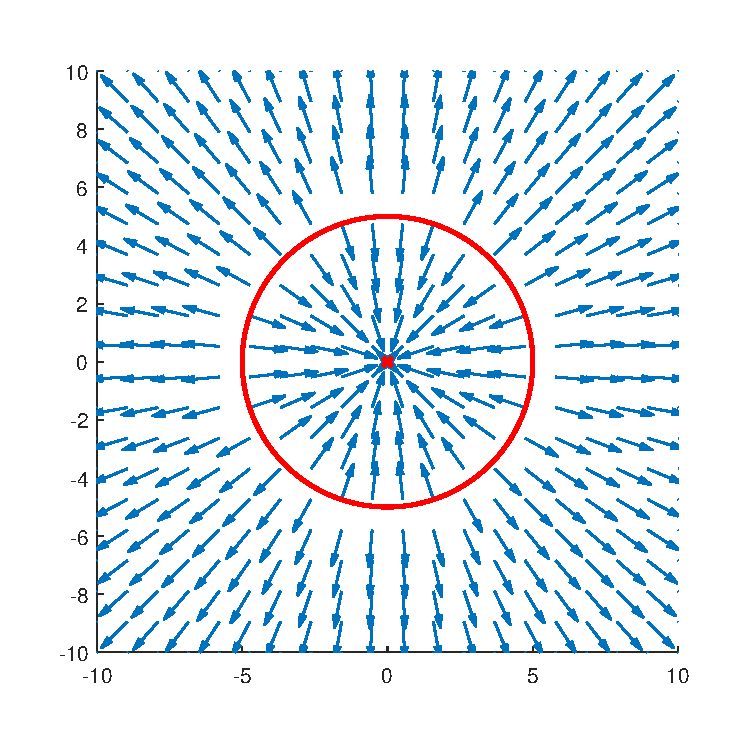
\includegraphics[width=6.5cm] {PaperFigures/compWithoutTitles/circRepulsive}}
%		\subfigure []{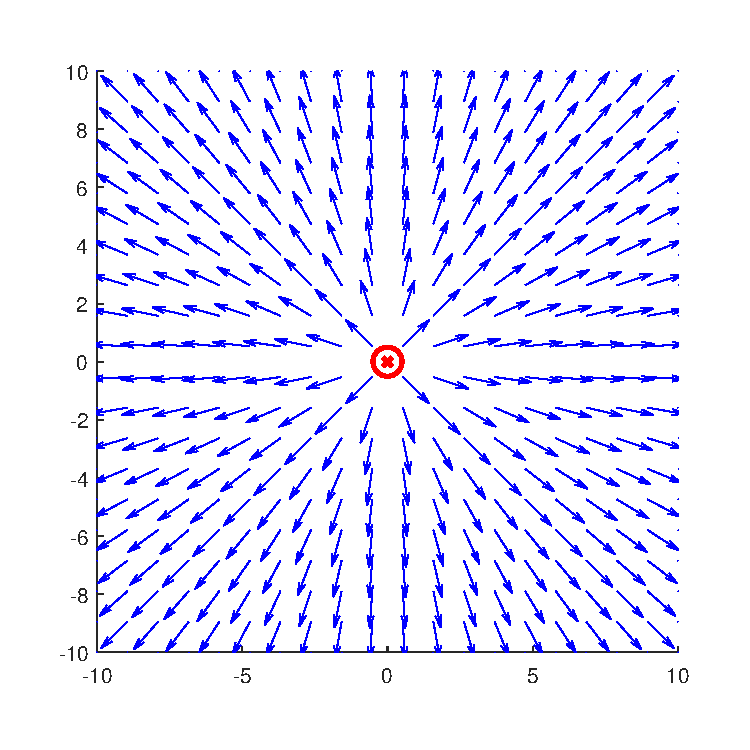
\includegraphics[width=6.5cm] {PaperFigures/compWithoutTitles/circRepulsiveSmallr}}
%		\hspace*{0mm}
%	\end{subfigmatrix}
%	\caption{Repulsive field with large path radius (a) and small radius (b)}
%	\label{fig:gvfRepulsiveRadius}
%\end{figure}
%
%The strength of the repulsive field was varied as a function of proximity $d$ by multiplying the repulsive field by a decay function $P$ bounded on the interval [-1,0], shown in Equation \ref{repulsiveDecay} and Figure \ref{fig:tanhICUAS2018}. The radius $R$ is the distance from the center of the field where vectors have effectively zero strength. 
%
%\begin{equation}
%P = R\frac{tanh(2\pi d-\pi)+1}{2}
%\label{repulsiveDecay}
%\end{equation}
%
%\begin{equation}
%\vec{v}_{repulsive} = -G||\vec{v_{conv}}||P
%\label{replulsiveField}
%\end{equation}
%
%
%
%\begin{figure}[H]
%	\begin{subfigmatrix}{2}% number of columns
%		\centering	
%		\subfigure []{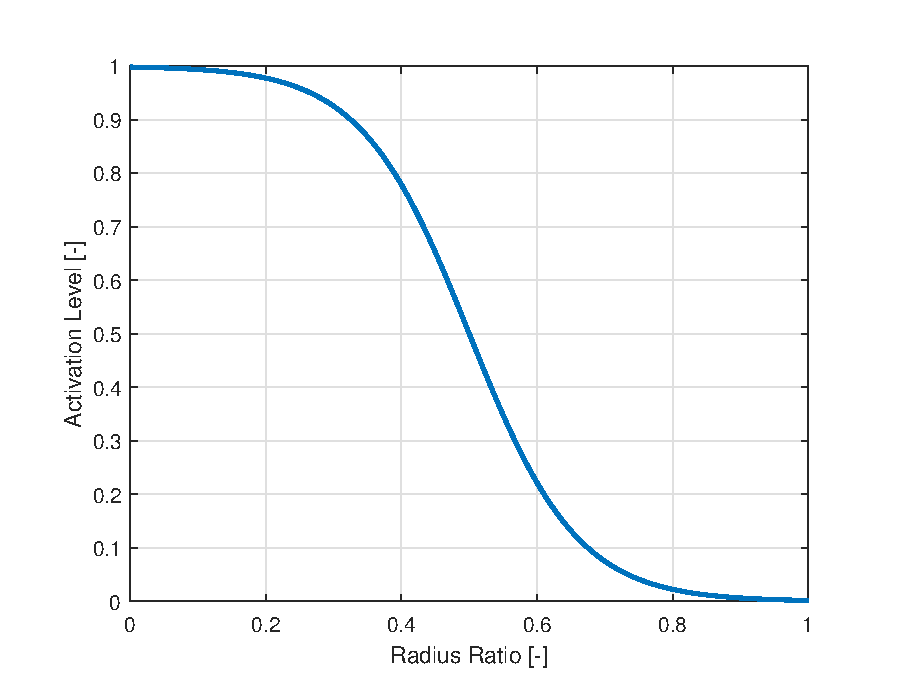
\includegraphics[width=8cm] {PaperFigures/tanh_ICUAS2018}}
%		\subfigure []{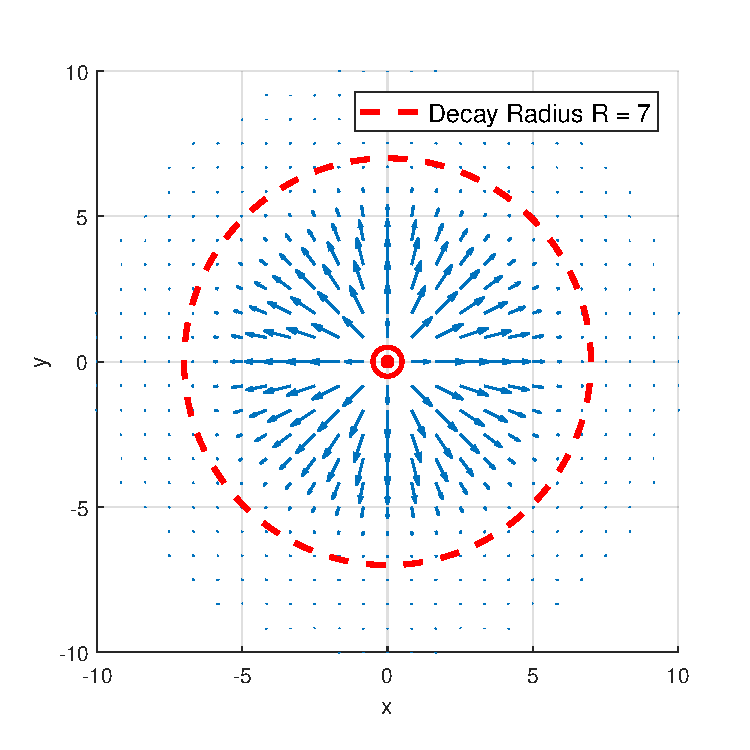
\includegraphics[width=7cm] {PaperFigures/repulsiveFields/circRepulsiveDecay}}
%		\hspace*{0mm}
%	\end{subfigmatrix}
%	\caption{Repulsive field activation \cite{wwc} (a) resulting repulsive field (b)}
%	\label{fig:tanhICUAS2018}
%\end{figure}
%
%
%Attractive and repulsive fields were added together similar to that in \cite{panagou_motion_2014} and the resulting vector shown in Equation \ref{summedAttRepulsive}. The resultant heading vector was used to guide a UAV to track a moving loiter circle while avoiding static obstacles, shown in Figure \ref{fig:gvfMovingTarget}.
%
%\begin{equation}
%\vec{V} = \vec{v}_{attractive}+\vec{v}_{repulsive}
%\label{summedAttRepulsive}
%\end{equation}
%
%
%
%\begin{figure}[h]
%	\centering
%	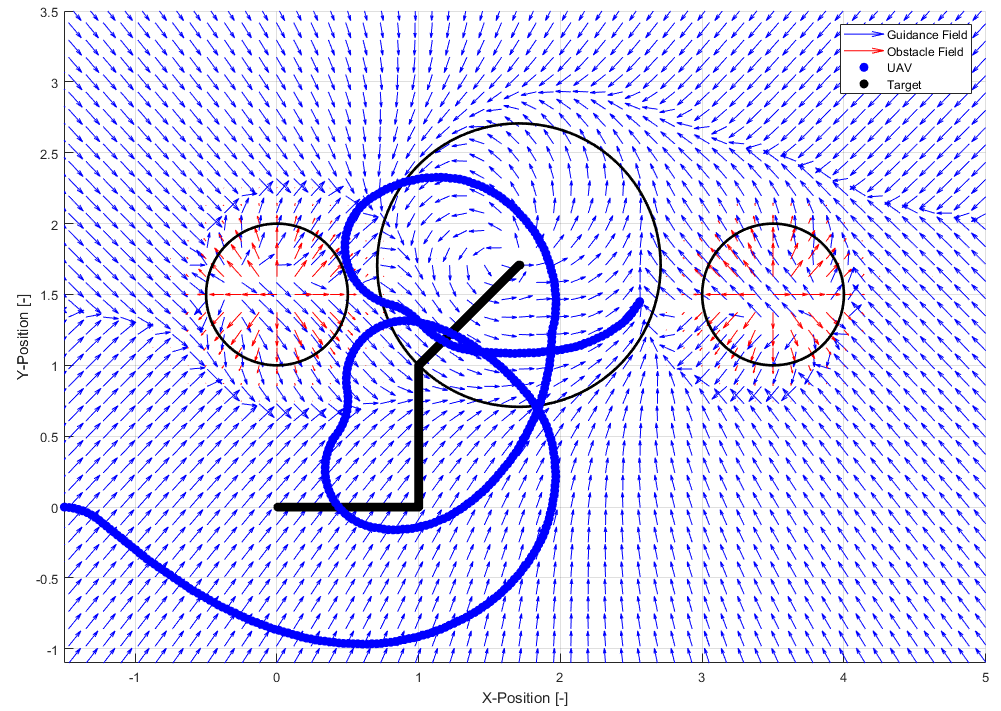
\includegraphics[width=10cm]{PaperFigures/gvfMovingTarget}
%	\caption{Place holder image of UAV following ground target \cite{wwc}}
%	\label{fig:gvfMovingTarget}
%\end{figure}
%
%
%GVF weights have been used for high level specification of the desired behavior for a UAV, whether it be for convergence, circulation, or avoidance. Repulsive GVFs have considered obstacle fields that strictly repel. The strictly repulsive guidance is effective at directing a UAV away from an obstacle, but provides no information on how to circumnavigate one. Additionally, further specification on the minimum radius and strength of the repulsive field may be useful in preventing a UAV from violating the obstacle circle. A preliminary simulation shows that a UAV encountering an obstacle while tracking a path may result in violation of the obstacle space, shown in Figure \ref{fig:singleobstacle}. UAVs traveling at lower velocities
%may also enter a trap situation where the guidance is confined to an infinite loop.
%\pagebreak
%
%\begin{figure}[h]
%	\centering
%	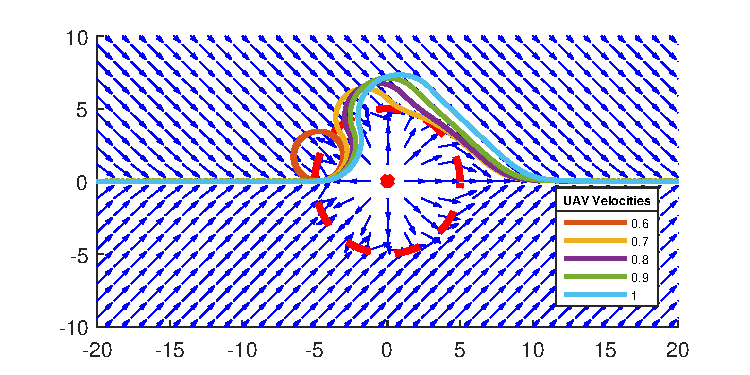
\includegraphics[width=12cm]{PaperFigures/singleObstacle}
%	\caption{Strictly repulsive obstacle on straight path}
%	\label{fig:singleobstacle}
%\end{figure}
%
%
%Adding circulation \textit{\textbf{H=1}} to the GVF in Figure \ref{fig:singleobstacle} prevented the trap situation for a velocity $u = 0.6$ and reduced the circumnavigation distance, which is shown in Figure \ref{fig:singleobstacleWithCirc}. Specifying vector field weights as functions of a UAV's state may enable an optimal guidance for obstacle avoidance. 
%
%\begin{figure}[h]
%	\centering
%	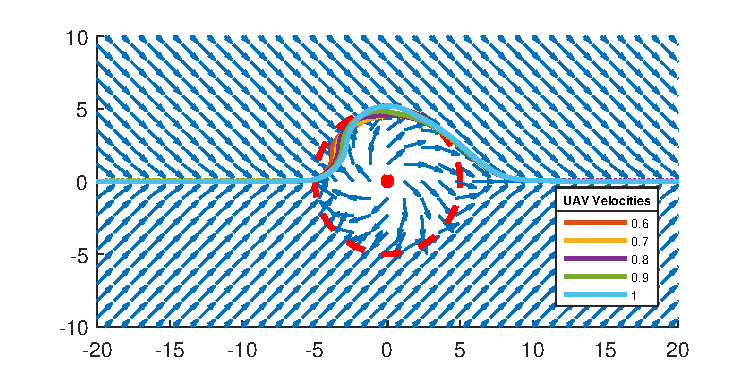
\includegraphics[width=12cm]{PaperFigures/singleObstacleWithCirc}
%	\caption{Circulating repulsive obstacle on straight path}
%	\label{fig:singleobstacleWithCirc}
%\end{figure}



\section{Literature Review Summary}


Vector fields can provide guidance and control for robots through the use of artificial attractive and repulsive forces. Converging to a singular point while avoiding obstacles can be achieved with Potential Field or Virtual Force Field methods. Fixed wing UAVs cannot converge to a singular point therefore vector fields that asymptotically converge and follow a path is beneficial. Lyapunov and Gradient Vector Fields have been used for path following, standoff tracking, and obstacle avoidance. Gradient Vector Field provides convenient and decoupled access to scalar multiplicative weights for the convergence, circulation, and time-varying terms. Negative weights can be used for obstacle avoidance, however have so far been used only as high level specification of guidance behavior. Specifying vector field weights as functions of a UAV's state may enable an optimal guidance for obstacle avoidance. Validation of a modified GVF guidance can be performed on mobile ground robots simulating UAV dynamics.

\chapter{Methodology}

%\section{Dubins Vehicle}
%The dynamics of UAVs are often simplified when simulating guidance systems by modeling the UAV as a Dubin's vehicle \cite{frew_cooperative_2007,griffiths_vector_2006,nelson_cooperative_2005,nelson_vector_2006,nelson_vector_2007}. It is assumed that the autopilots control system is capable of maintaining stability, speed $u$, and can turn the vehicle at a fixed turn rate $\dot{\theta}$. The position of the UAV $\overrightarrow{X}$ at time $t$ is calculated from the integral of the velocity vector $\overrightarrow{U}$, Equation \ref{eq:uavPosition}. Heading is an input from a guidance system, such as waypoint, potential field, or vector field.
%
%\begin{equation}
%\label{eq:uavVelocity}
%\overrightarrow{U}(t) = u \begin{bmatrix}
%cos(\theta(t)) \\
%sin(\theta(t))
%\end{bmatrix}
%\end{equation}
%
%
%\begin{equation}
%\label{eq:uavPosition}
%\overrightarrow{X}(t) = \overrightarrow{U}dt + \overrightarrow{X}(t-1)
%\end{equation}
%
%
%\begin{equation}
%\label{turnRate}
%\dot{\theta} \leq 20 deg/s
%\end{equation}


%\subsection{MOVE TO METHODOLOGY}
%The GVF weights are decoupled from each term calculation, therefore modifications to the GVF weights do not require a new derivation of the resulting field. Magnitude of the weights effectively scales the contribution of each term. Negating the GVF weights has been used to provide a repulsive field for obstacle avoidance in \cite{wwc} for a UAV tracking a moving loiter circle. Assigning weights \textbf{G=-1} and \textbf{H=L=0} rotates the attractive field vectors in Figure \ref{fig:gvfCircAttractive}b 180$^\circ$ about the tail of each vector, which is shown in Figure \ref{fig:gvfRepulsiveRadius}a. Note how the repulsive field vectors point away from the circular curve for the entire configuration space. Encircling an obstacle by a path produces vectors that may provide guidance into the obstacle, which is not desired. Reducing the radius to be smaller than the radius of the obstacle produces a GVF with nearly all vectors directing away. 
%
%
%\begin{figure}[H]
%	\begin{subfigmatrix}{2}% number of columns
%		\centering	
%		\subfigure []{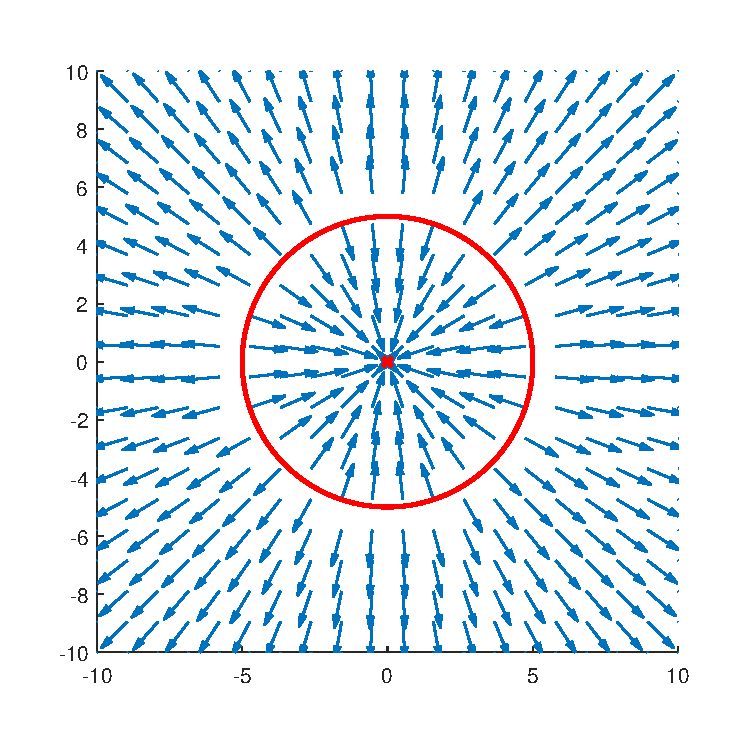
\includegraphics[width=6.5cm] {PaperFigures/compWithoutTitles/circRepulsive}}
%		\subfigure []{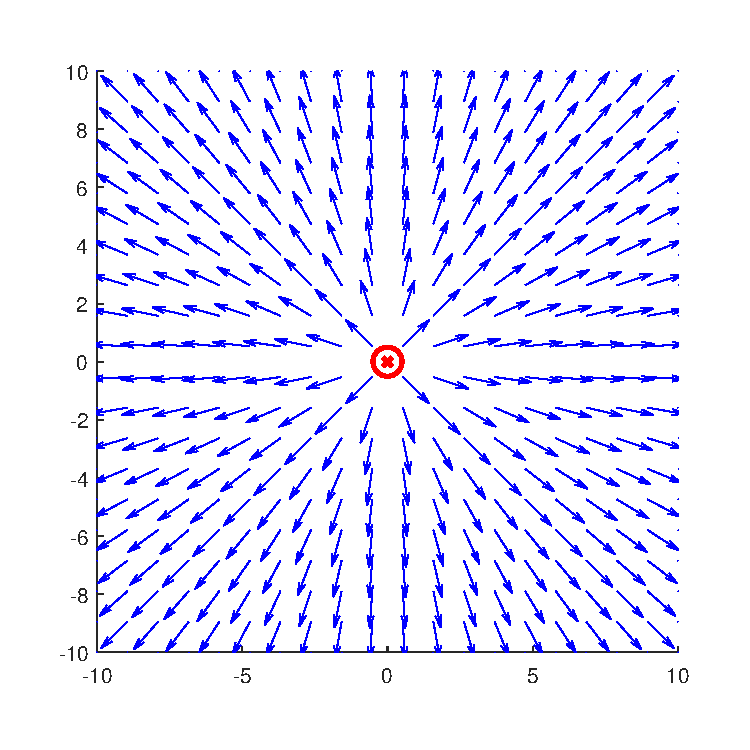
\includegraphics[width=6.5cm] {PaperFigures/compWithoutTitles/circRepulsiveSmallr}}
%		\hspace*{0mm}
%	\end{subfigmatrix}
%	\caption{Repulsive field with large path radius (a) and small radius (b)}
%	\label{fig:gvfRepulsiveRadius}
%\end{figure}
%
%The strength of the repulsive field was varied as a function of proximity $d$ by multiplying the repulsive field by a decay function $P$ bounded on the interval [-1,0], shown in Equation \ref{repulsiveDecay} and Figure \ref{fig:tanhICUAS2018}. The radius $R$ is the distance from the center of the field where vectors have effectively zero strength. 
%
%\begin{equation}
%P = R\frac{tanh(2\pi d-\pi)+1}{2}
%\label{repulsiveDecay}
%\end{equation}
%
%\begin{equation}
%\vec{v}_{repulsive} = -G||\vec{v_{conv}}||P
%\label{replulsiveField}
%\end{equation}
%
%
%
%\begin{figure}[H]
%	\begin{subfigmatrix}{2}% number of columns
%		\centering	
%		\subfigure []{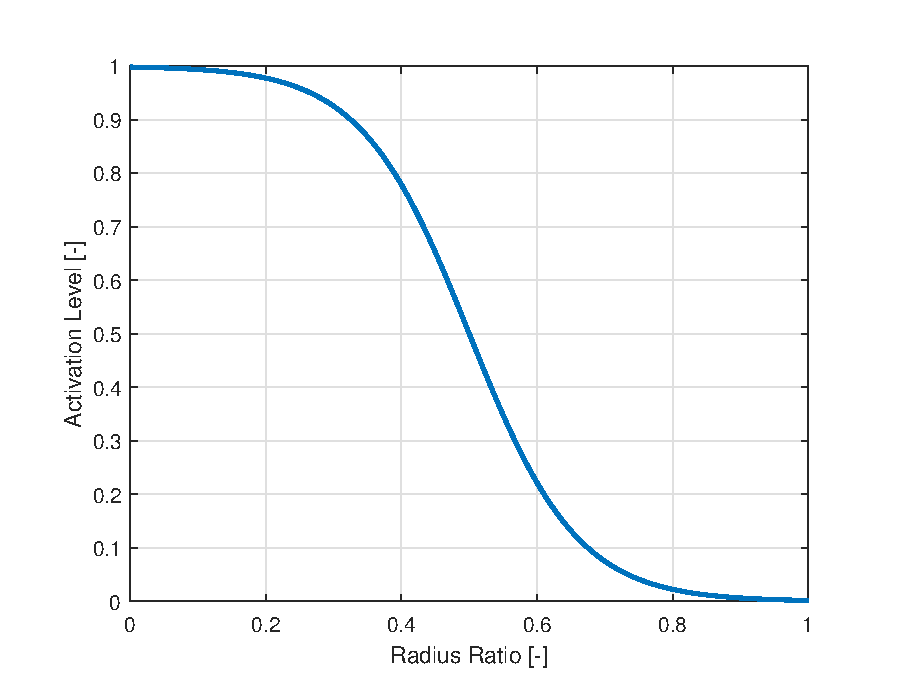
\includegraphics[width=8cm] {PaperFigures/tanh_ICUAS2018}}
%		\subfigure []{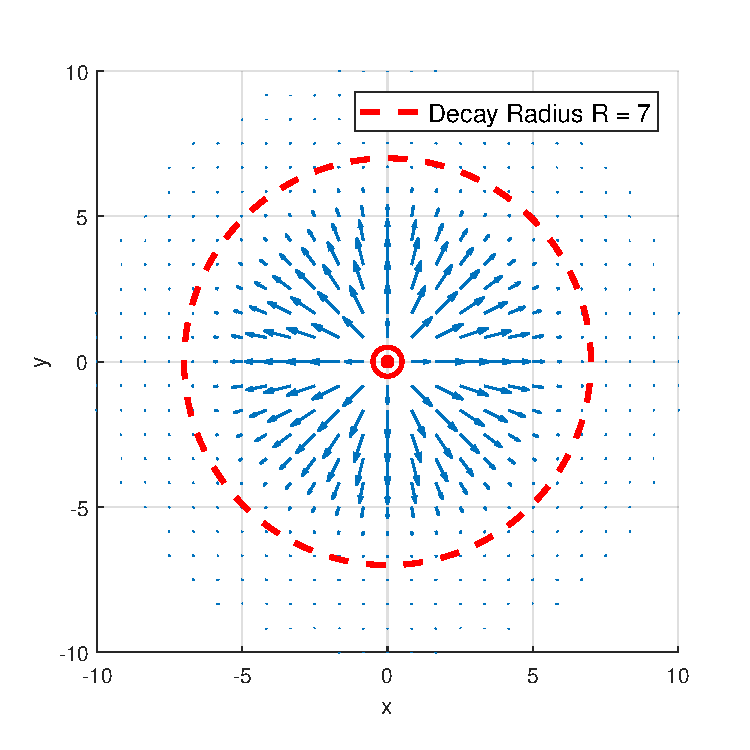
\includegraphics[width=7cm] {PaperFigures/repulsiveFields/circRepulsiveDecay}}
%		\hspace*{0mm}
%	\end{subfigmatrix}
%	\caption{Repulsive field activation \cite{wwc} (a) resulting repulsive field (b)}
%	\label{fig:tanhICUAS2018}
%\end{figure}
%
%
%Attractive and repulsive fields were added together similar to that in \cite{panagou_motion_2014} and the resulting vector shown in Equation \ref{summedAttRepulsive}. The resultant heading vector was used to guide a UAV to track a moving loiter circle while avoiding static obstacles, shown in Figure \ref{fig:gvfMovingTarget}.
%
%\begin{equation}
%\vec{V} = \vec{v}_{attractive}+\vec{v}_{repulsive}
%\label{summedAttRepulsive}
%\end{equation}
%
%
%
%\begin{figure}[h]
%	\centering
%	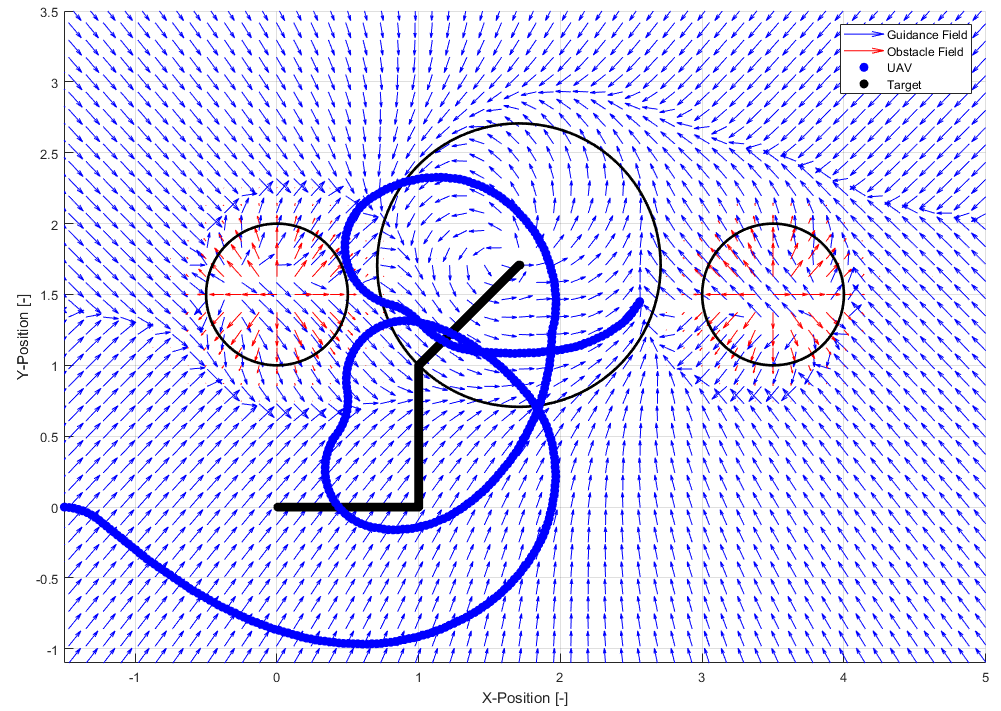
\includegraphics[width=10cm]{PaperFigures/gvfMovingTarget}
%	\caption{Place holder image of UAV following ground target \cite{wwc}}
%	\label{fig:gvfMovingTarget}
%\end{figure}
%
%
%GVF weights have been used for high level specification of the desired behavior for a UAV, whether it be for convergence, circulation, or avoidance. Repulsive GVFs have considered obstacle fields that strictly repel. The strictly repulsive guidance is effective at directing a UAV away from an obstacle, but provides no information on how to circumnavigate one. Additionally, further specification on the minimum radius and strength of the repulsive field may be useful in preventing a UAV from violating the obstacle circle. A preliminary simulation shows that a UAV encountering an obstacle while tracking a path may result in violation of the obstacle space, shown in Figure \ref{fig:singleobstacle}. UAVs traveling at lower velocities
% may also enter a trap situation where the guidance is confined to an infinite loop.
% \pagebreak
%
%\begin{figure}[h]
%	\centering
%	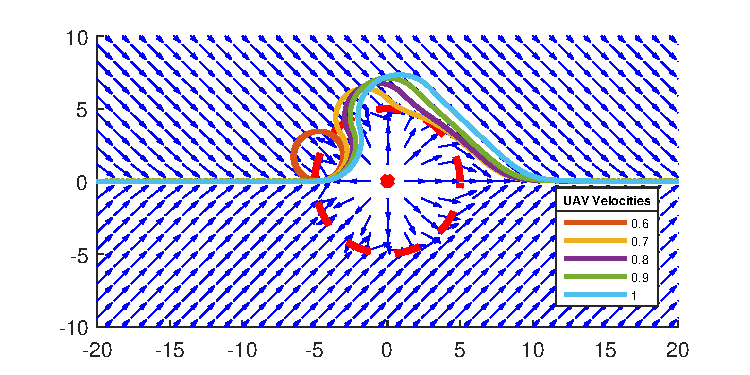
\includegraphics[width=12cm]{PaperFigures/singleObstacle}
%	\caption{Strictly repulsive obstacle on straight path}
%	\label{fig:singleobstacle}
%\end{figure}
%
%
%Adding circulation \textit{\textbf{H=1}} to the GVF in Figure \ref{fig:singleobstacle} prevented the trap situation for a velocity $u = 0.6$ and reduced the circumnavigation distance, which is shown in Figure \ref{fig:singleobstacleWithCirc}. Specifying vector field weights as functions of a UAV's state may enable an optimal guidance for obstacle avoidance. 
%
%\begin{figure}[h]
%	\centering
%	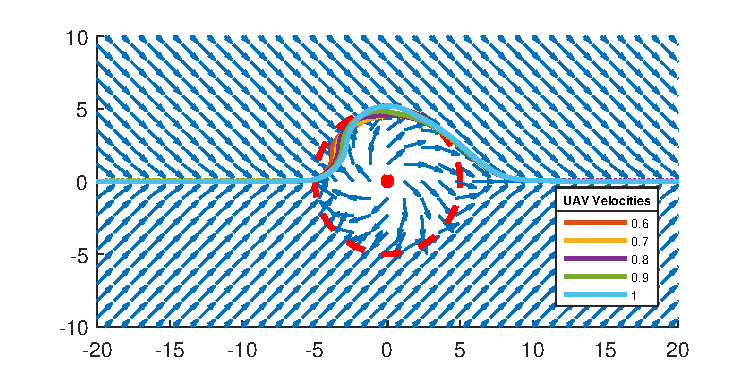
\includegraphics[width=12cm]{PaperFigures/singleObstacleWithCirc}
%	\caption{Circulating repulsive obstacle on straight path}
%	\label{fig:singleobstacleWithCirc}
%\end{figure}
%



%\pagebreak
%\section{Unmanned Aerial Vehicle Simulation}
%Testing new guidance, navigation, and control algorithms on flight hardware can be costly, require significant time, and requires an adequately large airspace. Before spending the time to reserve airspace and allocate man hours for flight tests it is important to test algorithms in a controlled environment. One way to accomplish testing without actual flight is through validation through mobile robots simulating fixed wing constraints \cite{ren_experimental_2007}, \cite{louali_designing_2014}, \cite{louali_experimental_2016}. Vector fields have been used in robot platforms other than UAVs, including ground \cite{kapitanyuk_guiding_2017} and marine \cite{schmitt_obstacle_2016}.
%
%\begin{figure}
%	\centering
%	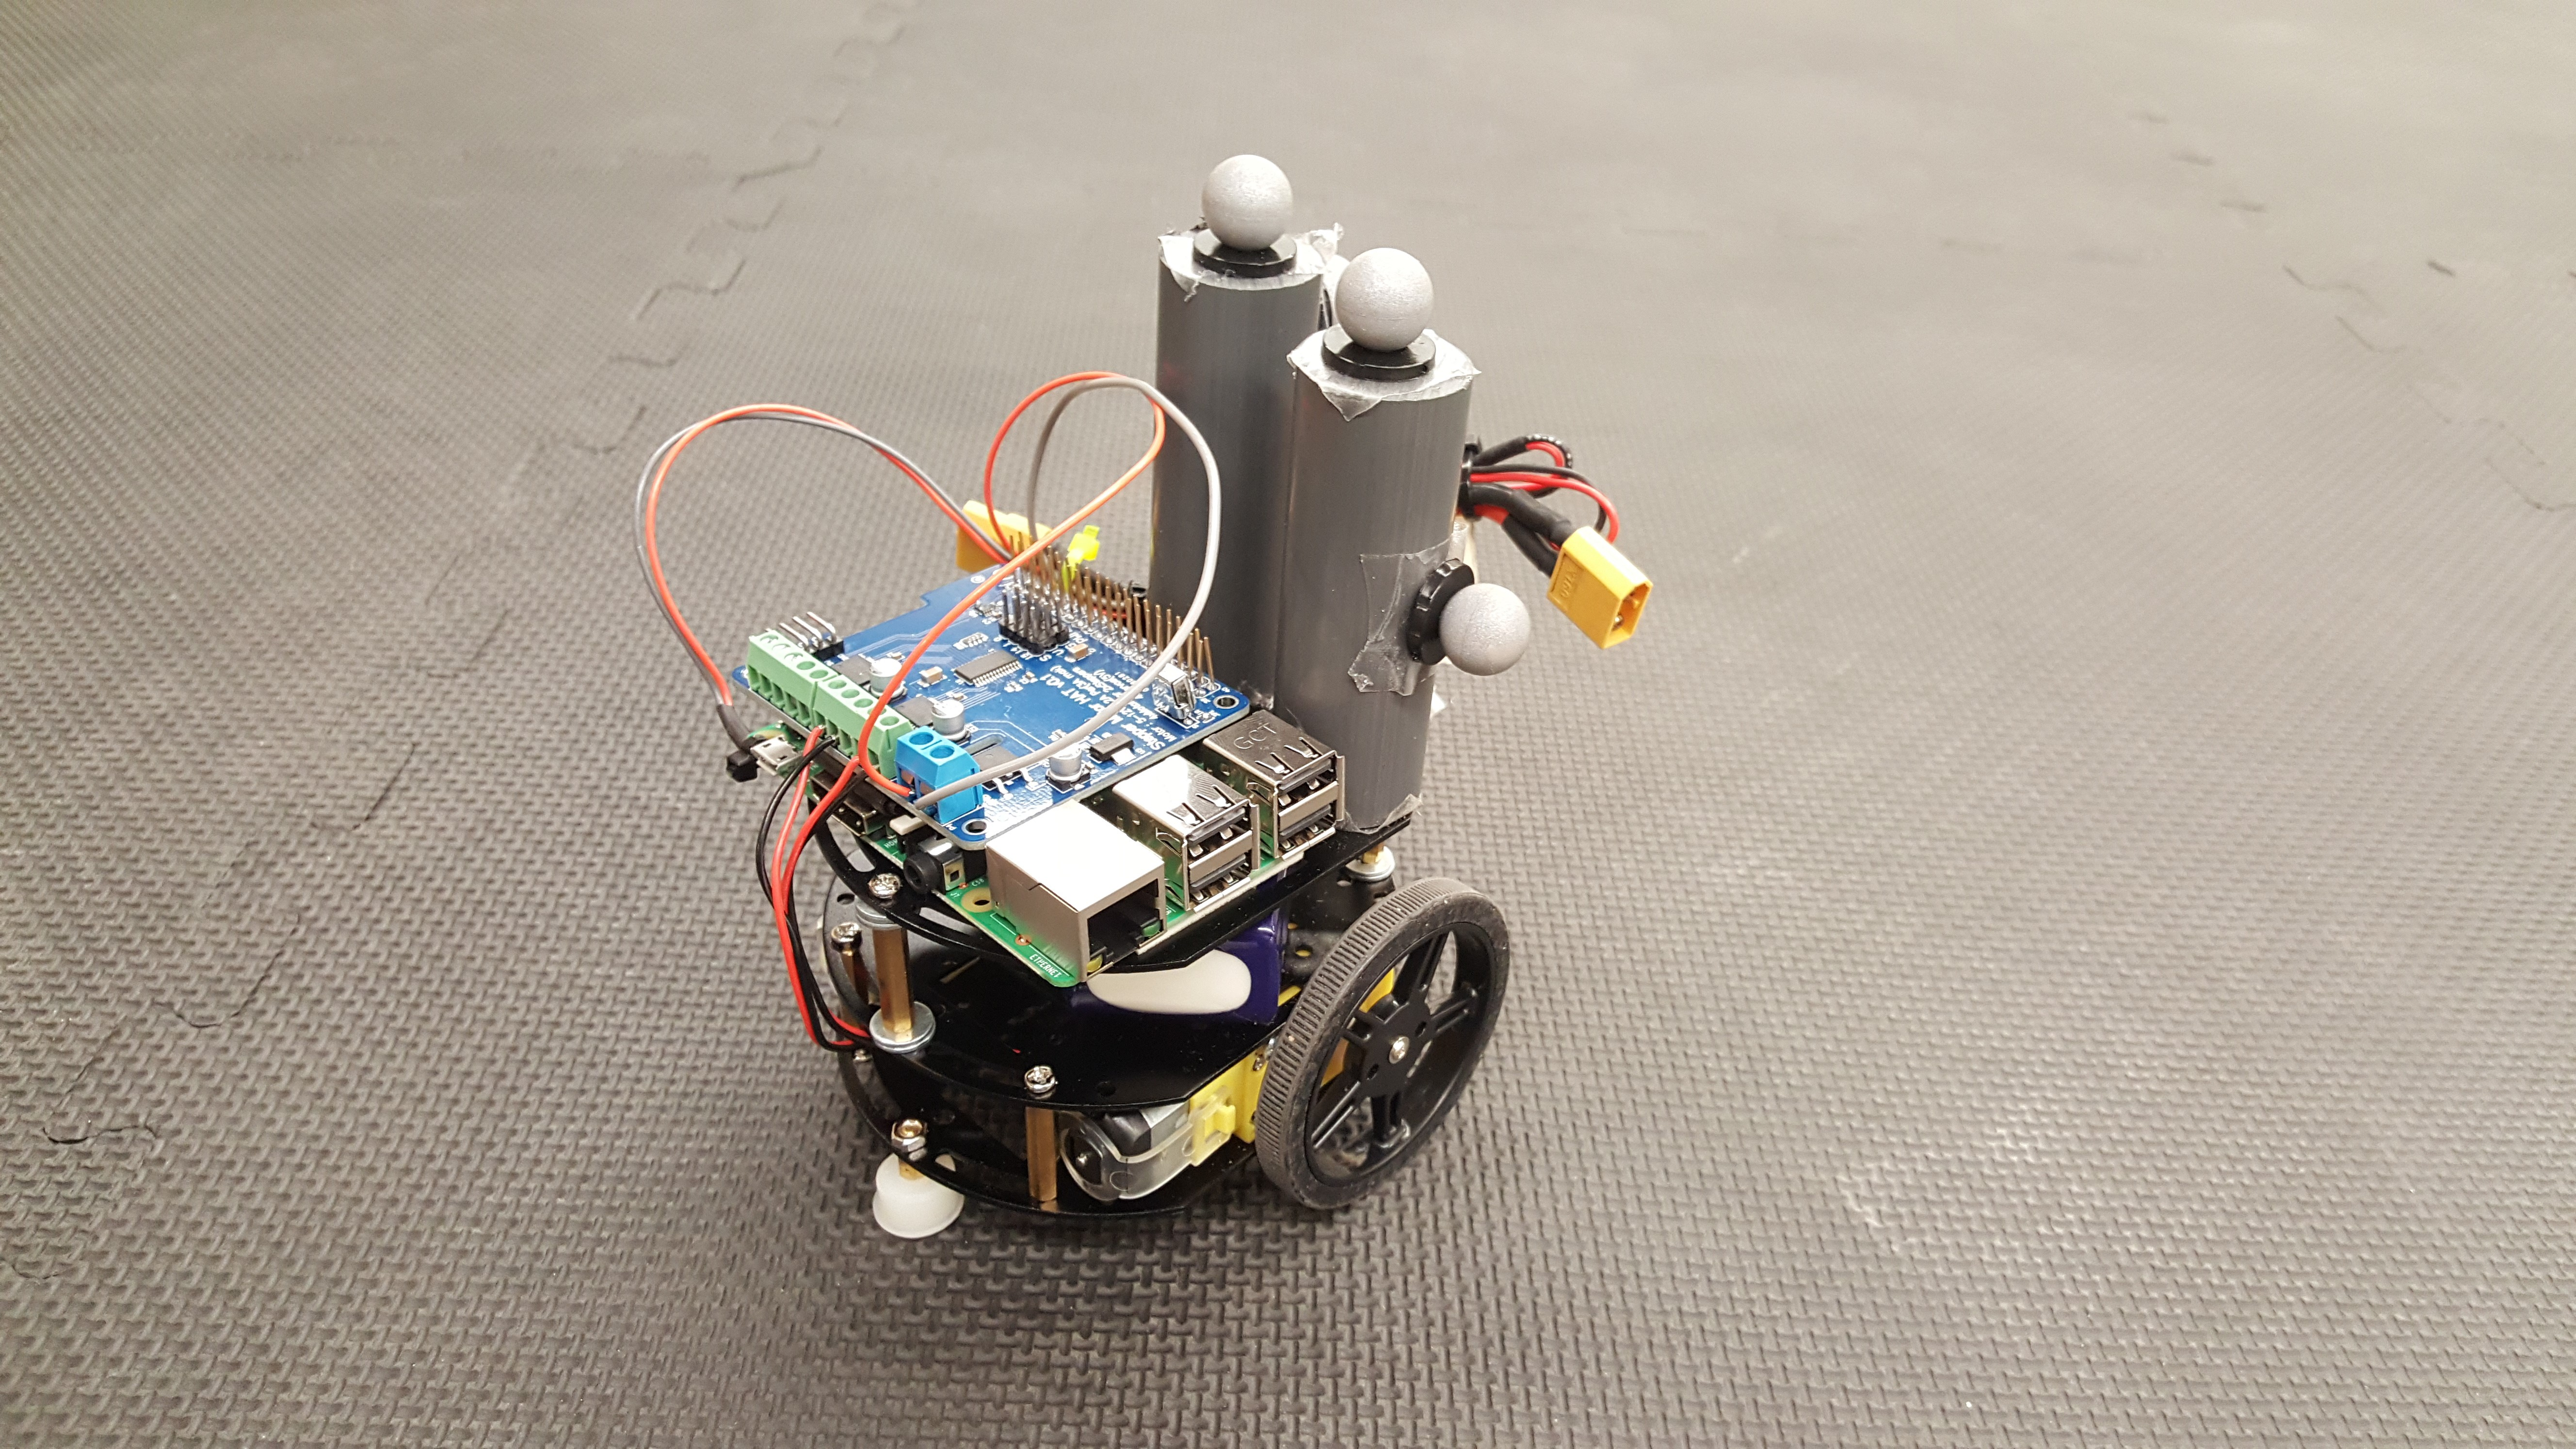
\includegraphics[width=15cm]{PaperFigures/robot}
%	\caption{Differential drive mobile robot simulating fixed wing UAV Dubins constraints}
%	\label{fig:robot}
%\end{figure}



\section{Introduction to Methodology}
A real-time circular obstacle avoidance guidance is achieved by summing together a path following and obstacle avoidance vector field with optimized decay and circulation weights. Singularities in summed vector fields are defined and a method for numerically locating their position is presented in Phase I and it is shown how adding circulation to repulsive GVFs may remove singularities from the UAVs path. Phase II investigates a method for selecting the combination of repulsive GVF decay radius and circulation weights that minimizes a path deviation cost function. The optimized GVF guidance is implemented on an indoor multirotor UAV operating under fixed wing constraints in Phase III.


\section{Phase I: Gradient vector field singularity detection}
 \textbf{The objective of Phase I is to characterize and present a method for locating singularities in a summed gradient vector field in simulation.} Phase I consists of calculating guidance for converging and following a straight path using the GVF method in literature. An obstacle field is constructed for avoiding circular obstacles along the path by modifying GVF's convergence and circulation weights. Summing the attractive and repulsive GVFs results in guidance that guides the UAV along the planned path while pushing away from an obstacle. Regions in the summed guidance where the path following and obstacle guidance directly oppose each other, called singularities, result in vectors of zero length. A method for identifying the location of singularities is presented along with a method for mitigating them. 
 

\subsection{Path Following Vector Field Guidance}
Guidance for converging and following a path using GVF guidance is achieved by summing together convergence and circulation terms that are multiplied by scalars $G$ and $H$ respectively, shown in Equation \ref{eq:GVFNoTV}. The potential function $V$, Equation \ref{eq:potV} decreases asymptotically to null when approaching the target path and therefore the convergence vector begins to decrease as well. As the potential function decreases, the circulation term begins to dominate the guidance, promoting path following. How close to the target path the transition between convergence and circulation depends on the scalar weights $G$ and $H$ respectively. 


\begin{equation}\label{eq:GVFNoTV}
\overrightarrow{V} = G \nabla V + H(\nabla\alpha_1 \times \nabla\alpha_2)
\end{equation}

\begin{equation}
V = -\sqrt{{\alpha_1}^2 + {\alpha_2}^2}
\label{eq:potV}
\end{equation}



Equation \ref{eq:GVFNoTV} for straight path following will be represented in component form for convenience, shown in Equation \ref{gonAllCompNormalized}. The total vector $\overrightarrow{V}_p$ represents the non-normalized attractive path following vector comprised of both convergence and circulation terms. 

\begin{equation}
% Component vector field with conv and circ
\overrightarrow{V}_{p} = G \overrightarrow{V}_{conv} +H\overrightarrow{V}_{circ}
\label{gonAllCompNormalized}
\end{equation}

The shape of the target path that the vectors converge and follow depend on the specification of the implicit 3-dimensional surface functions $\alpha_1$ and $\alpha_2$. Intersecting two planes, shown in Figure \ref{fig:planeIntersection}, can be used to generate a GVF that converges and follows a straight path. The vertical plane, described in Equation \ref{eq:pathFunction}, at angle $\delta$ is intersecting with a horizontal plane at constant height $z$, Equation \ref{eq:pathFunctionZ}

\begin{figure}[H]
	\centering
	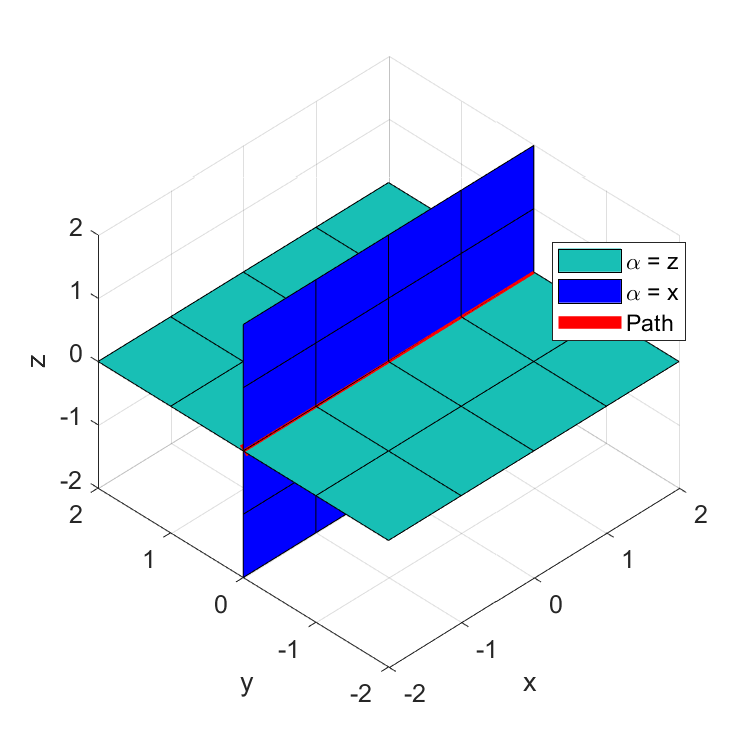
\includegraphics[width=8cm]{Figures/planeIntersection}
	\caption{Intersection of planes defined by implicit surface functions}
	\label{fig:planeIntersection}
\end{figure}



\begin{equation}
\label{eq:pathFunction}
\alpha_1 = cos(\delta)x + sin(\delta)y
\end{equation}

\begin{equation}
\label{eq:pathFunctionZ}
\alpha_2 = z
\end{equation}

\noindent
The gradient potential, $\nabla V$, for calculating the path following convergence term is shown in Equation \ref{eq:potentialFunctionGrad}.

\begin{equation}
\label{eq:potentialFunctionGrad}
\nabla V = -\frac{1}{2(\sqrt{\cos^2(\delta) x^2+2\cos(\delta)\sin(\delta) xy +\sin^2 (\delta) y^2})} \begin{bmatrix}
2x\cos^2(\delta) + 2\cos(\delta)\sin(\delta) y \\
2y\sin^2(\delta) + 2\cos(\delta)\sin(\delta) x \\
2
\end{bmatrix}
\end{equation}

\noindent
Circulation is calculated by the cross product of the surface function gradients, which evaluates to that shown in Equation \ref{eq:circStraightPart2}.


\begin{equation}
\label{eq:circStraightPart2}
\overrightarrow{V}_{circ} = \begin{bmatrix}
sin(\delta) \\
-cos(\delta) \\
0
\end{bmatrix}
\end{equation}

Prior to using the path following guidance $\overrightarrow{V}_p$, it is normalized to have a magnitude $||\overrightarrow{V}_p|| = 1$. The reason for normalizing the vector is threefold. First, the vector is used as a heading controller only, therefore the angle of the vector is the necessary information. Second, the normalized vectors result in quiver plots with equal density arrows making the field easier to visualize. Lastly, normalizing the path following vector $\overrightarrow{V}_p$ fixes the length of the vector allowing for prediction of singularity location after summing the field, which will be discussed in the next section. Before discussing singularities, the obstacle field is introduced. 


\begin{equation}
% Component vector field with conv and circ
\overrightarrow{V}_{||P||} = \frac{\overrightarrow{V}_p}{||\overrightarrow{V}_p||}
\label{gonAllCompNormalized}
\end{equation}

To produce guidance for following a path and avoiding an obstacle, a repulsive obstacle vector field $\overrightarrow{V}_{||O||}$ needs to be constructed and summed with the normalized path following guidance $\overrightarrow{V}_{||P||}$. The repulsive vector field is multiplied by a decay function $P$ which limits the influence of the obstacle to a finite range and will be discussed after the avoidance field equations are presented. The sum of the two guidances is represented by $\overrightarrow{V}_g$ and is shown in Equation \ref{eq:totalGuidance}


\begin{equation}
\label{eq:totalGuidance}
\overrightarrow{V}_g = \overrightarrow{V}_{||P||} + P\overrightarrow{V}_{||O||}
\end{equation}

\noindent
Constructing the obstacle avoidance vector field will now be discussed.

\subsection{Constructing an Avoidance Vector Field}

A circular avoidance vector field will now be constructed in a way similar to that of the path following field in the previous section. What differentiates the obstacle field from the path following field is that the individual convergence and circulation components are normalized prior to normalizing the summed obstacle field $\overrightarrow{V}_o$. The benefit of normalized each field component before multiplying by their respective scalars and summing is to produce a obstacle field with uniform behavior as distance from the obstacle increases. In short, normalizing each component allows both convergence and circulation terms to be present in the obstacle guidance at larger distances. Additionally, negative convergence weights will be used to produce vectors that diverge away from the path. The obstacle vector field is constructed using the normalized component Equation \ref{eq:obstComponents} with obstacle convergence and circulation weights $G_o$ and $H_o$ respectively.


\begin{equation}
% Component vector field with conv and circ
\overrightarrow{V}_{o} = G_o\frac{\overrightarrow{V}_{conv}}{||\overrightarrow{V}_{conv}||}+H_o\frac{\overrightarrow{V}_{circ}}{||\overrightarrow{V}_{circ}||}
\label{eq:obstComponents}
\end{equation}



A circular avoidance vector field with radius $r$ centered at $(x_c,y_c)$ is constructed by intersecting a cylinder, Equation \ref{eq:alphaCylinder}, and a plane Equation \ref{eq:pathFunctionZ}. 

\begin{equation}\label{eq:alphaCylinder}
\alpha_1 = (x-x_c)^2 + (y-y_c)^2-r^2
\end{equation}


\begin{figure}[H]
	\centering
	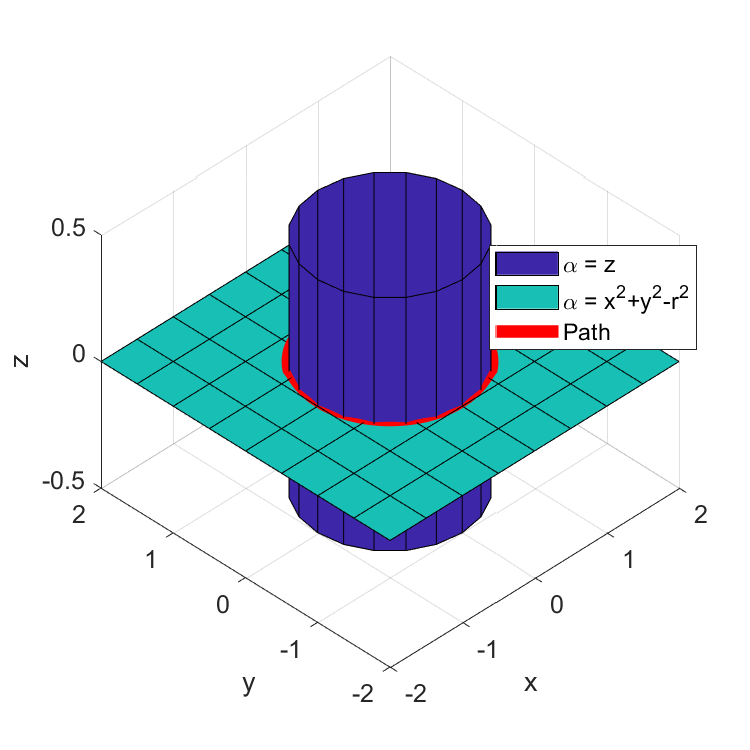
\includegraphics[width=10cm]{Figures/cylinderIntersection}
	\caption{Intersection of a cylinder and plane defined by implicit surface functions}
	\label{fig:cylinderIntersection}
\end{figure}



Convergence is calculated by the gradient of the potential function \ref{eq:potentialFunctionGrad}, which when simplified evaluates to

\begin{equation}
\nabla V = A\overrightarrow{B}
\label{eq:AB}
\end{equation}

\noindent
where


\begin{equation}
A = \dfrac{-1}{\sqrt{\bar{x}^4+\bar{y}^4+2\bar{x}^2\bar{y}^2-2r^2\bar{x}^2-2r^2\bar{y}^2+r^2+z^2}}
\end{equation}

\begin{equation}
\overrightarrow{B} = \begin{bmatrix} 2\bar{x}^3+2\bar{x}\bar{y}^2-2r^2\bar{x} \\ 2\bar{y}^3+2\bar{x}^2\bar{y}-2r^2\bar{y} \\z \end{bmatrix}
\end{equation}

\noindent
and


\begin{equation}
\bar{x} = x - x_c
\end{equation}
\begin{equation}
\bar{y} = y - y_c
\end{equation}


Evaluating equation \ref{eq:AB} results in a vector field that converges to a circular path. Circulation is calculated from the cross product of each implicit surface function's gradient, which simplifies to



\begin{equation}\label{eq:vcirc_circle}
\overrightarrow{V}_{circ} =  \begin{bmatrix}  2(y-y_c) \\[6pt] -2(x-x_c) \\[6pt] 0\end{bmatrix}
\end{equation}

Obstacle fields should only act locally on a UAV guidance which is accomplished by applying a decay function for a field of radius $R$. The decay strength $P$ is determined in \ref{eq:decay}, where $d$ is the euclidean distance, or range, between the UAV and the center of the obstacle, shown in Equation \ref{eq:range}. At a distance $d>R$ the decay strength $P$ is effectively zero, having virtual no influence on the total guidance. At a distance $d\leq R$, the field strength is bounded between $[0,2]$. The selection of the decay function $P$ to be bounded as such is so that the obstacle field $\overrightarrow{V}_o$ eventually overpowers the path field $\overrightarrow{V}_{||P||}$. A plot of the decay function in Equation \ref{eq:decay} is shown in Figure \ref{eq:range}.


\begin{equation}
\label{eq:decay}
P = -\tanh \bigg( \frac{2\pi d}{R}-\pi\bigg)+1
\end{equation}

\begin{equation}
\label{eq:range}
d = \sqrt{ \bar{x}^2+\bar{y}^2}
\end{equation}

\begin{figure}[H]
	\centering
	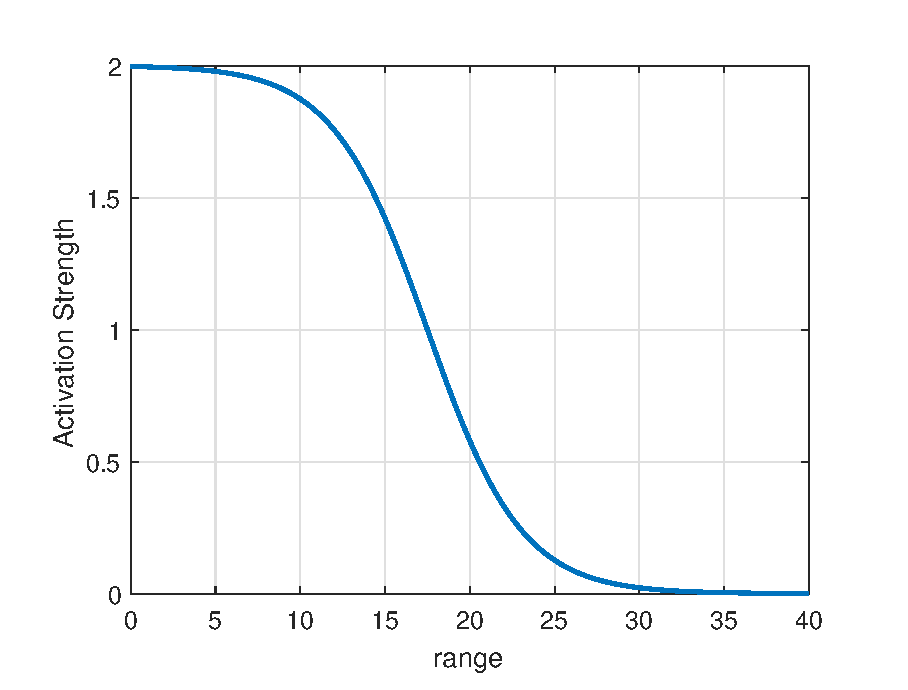
\includegraphics[width=0.7\linewidth]{Figures/methods/tanH}
	\caption{Repulsive GVF decay function P}
	\label{fig:tanh}
\end{figure}

Prior to applying the decay function the sum of obstacle field's convergence and circulation terms are normalized to ensure the vector's magnitudes are of length unity, shown in Equation \ref{eq:obstNormalized}.


\begin{equation}
% Component vector field with conv and circ
\overrightarrow{V}_{||o||} = \frac{\overrightarrow{V}_{o}}{||\overrightarrow{V}_{o}||}
\label{eq:obstNormalized}
\end{equation}


\subsection{Summed Guidance and Singularity Definition}
The total summed guidance $\overrightarrow{V}_g$ defined in Equation \ref{eq:totalGuidance} can now be calculated and visualized, Figure \ref{fig:summedFieldsNoNorm}. In general, the GVF guidance is more easily visualized if the final guidance is normalized yet again, however, plotting the path following and obstacle guidance $\overrightarrow{V}_g$ demonstrates regions where the fields oppose each other, possibly leading to GVF singularities. For a strictly repulsive field that is centered on a straight path, regions of both constructive and destructive summation occurs. Note the vectors on the positive x-axis increasing in length as the two fields come together. Conversely, vectors in the negative x-axis show decreasing length and in some areas disappearing entirely.  

\begin{figure}[H]
	\centering
	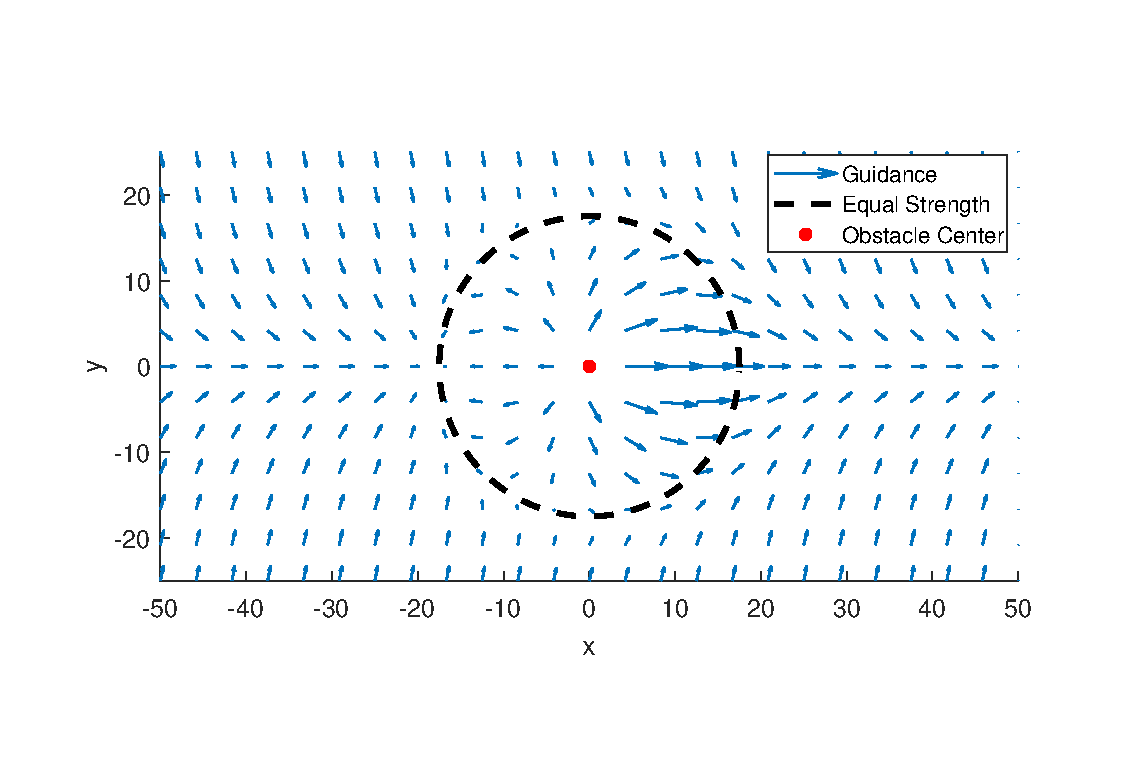
\includegraphics[trim=25 35 25 50,clip,width=14cm]{PaperFigures/Methods/summedFieldsNoNorm}
	\caption{Summed fields without total normalization $\protect \overrightarrow{V}_g$}
	\label{fig:summedFieldsNoNorm}
\end{figure}

It appears that the regions leading up to the singularities have vectors that guide towards the singularities. Opposing vectors that lead into a well may produce trap situations where a UAV may be unable to escape if continuing to use GVF guidance. The location of the singularities can be approximated by plotting the magnitude of the summed field near the obstacle. 

\begin{figure}[H]
	\centering
	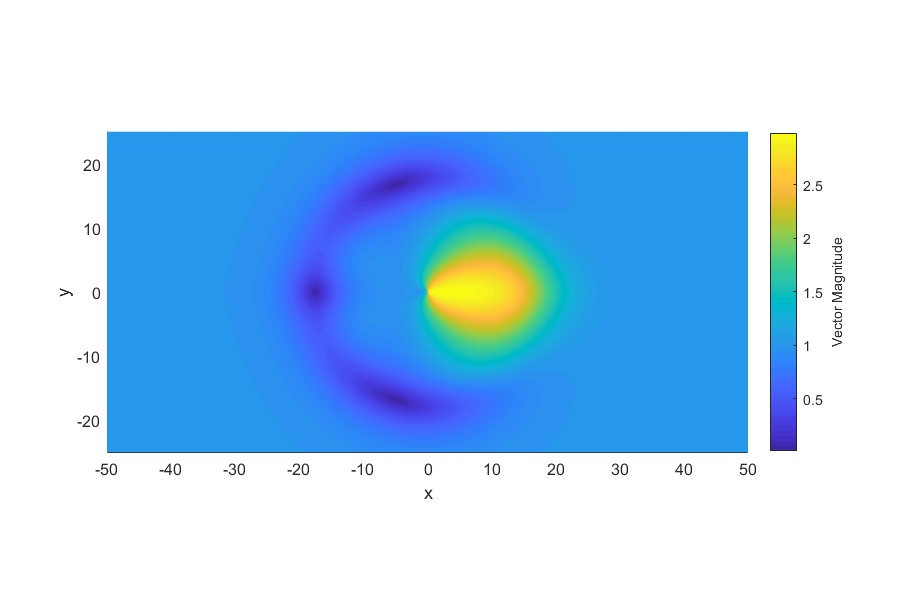
\includegraphics[trim=25 60 25 85,clip,width=14cm]{Figures/methods/summedHeatMapSimple}
	\caption{Summed Fields Without Total Normalization}
	\label{fig:summedHeatMap}
\end{figure}

 Singularities may be used to detect these regions and possibly protect UAVs from entering trap situations. Singularities in the vector field are defined as a region in the GVF space where the vector has zero magnitude, shown in Equation \ref{eq:singularityCondition}.


\begin{equation}
\label{eq:singularityCondition}
||\overrightarrow{V}_g || = 0
\end{equation}

\noindent
By extension, singularities are a result of a zero vector, shown in Equation \ref{eq:zeroVectorCondition} and Equation \ref{eq:zeroVectorCondition2}.



\begin{equation}
\label{eq:zeroVectorCondition}
\overrightarrow{0} = \overrightarrow{V}_{||P||} +P\overrightarrow{V}_{||O||}
\end{equation}

\begin{equation}
\label{eq:zeroVectorCondition2}
\overrightarrow{V}_{||P||}=-P\overrightarrow{V}_{||O||}
\end{equation}

Vectors $\overrightarrow{V}_{||P||}$ and $\overrightarrow{V}_{||O||}$ are normalized, meaning that their magnitudes are of equal length $||\overrightarrow{V}_{||P||}||=||\overrightarrow{V}_{||O||}||$. For the condition shown in Equation \ref{eq:zeroVectorCondition2} to be true for an obstacle field with a negative convergence weight $G=-1$, the decay function $P$ must be unity. Setting Equation \ref{eq:decay} equal to $1$, the distance at which the fields have equal strength is determined to be that shown in Equation \ref{eq:equalStrength}

\begin{equation}
\label{eq:equalStrength}
d = \frac{R}{2}
\end{equation}

An example of using a numerical solver with various initial conditions placed along a radius of $d=r/2$ is shown in Figure \ref{fig:noCircSingularityDetection}


\begin{figure}[H]
	\begin{subfigmatrix}{2}% number of columns
		\centering	
		\subfigure []{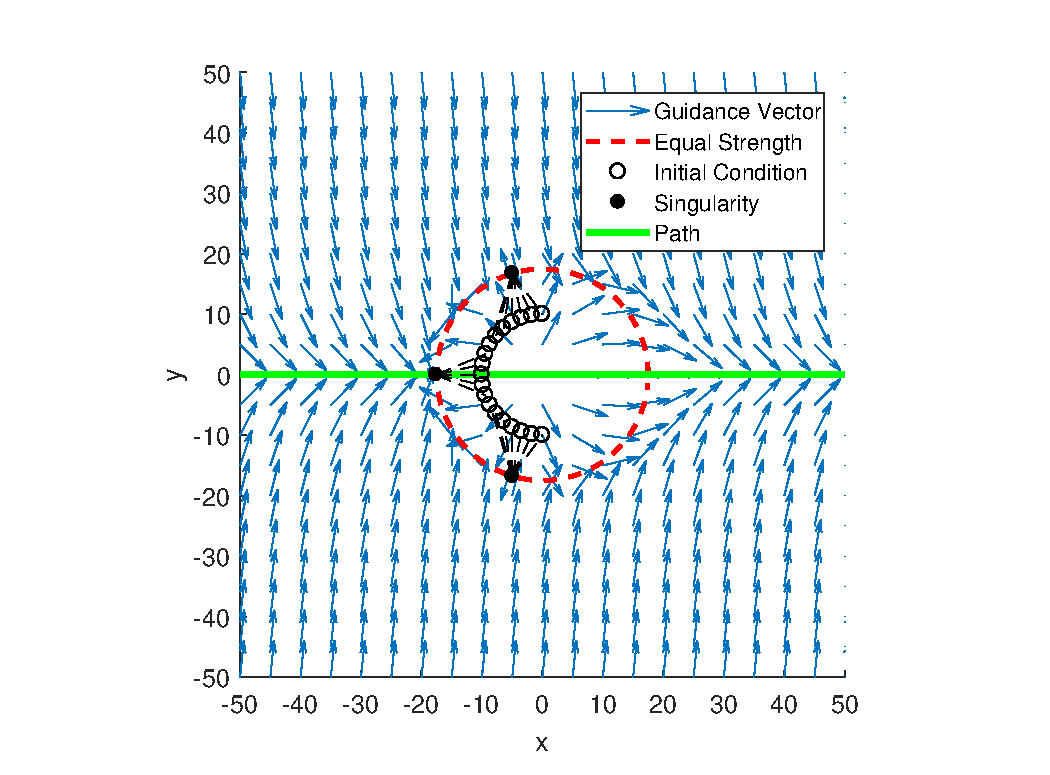
\includegraphics[trim=70 0 80 0,clip,width=7cm] {Figures/methods/noCircSingularityR10}}
		\subfigure []{\includegraphics[trim=70 0 80 0,clip,width=7cm] {Figures/methods/noCircSingularityR30}}
		\hspace*{0mm}
	\end{subfigmatrix}
	\caption{GVF converging and circulating circular path}
	\label{fig:noCircSingularityDetection}
\end{figure}

The method for constructing path following and obstacle GVFs will be used in Phase II along with singularity detection.




%\subsection{Summary of Phase I}
%GVF equations were derived for straight path following and circular obstacle avoidance. Singularities and their expected location within a summed field were characterized. A method for detecting GVF singularities numerically was presented. Circulation was added to the repulsive GVF to demonstrate the mitigation of GVF singularities. A method for selecting GVF obstacle radius and circulation strength will be discussed next.
%
%
%A cost function for evaluating GVF performance for obstacle avoidance is presented. Justification for selecting which GVF weighting parameters is provided. An evaluation of multiple parameters for a worst case encounter is described and the effect on cost discussed. 

\pagebreak

\section{Phase II: Optimization of Obstacle Field}
\textbf{The objective of Phase II is to determine a combination of circulation and decay radius for a circular obstacle GVF that produces an optimized obstacle avoidance.} Phase II consists of presenting a Dubin's fixed wing UAV kinematics to be used in simulating the GVF guidance. 
A demonstration of the modeled UAV converging and following a straight path for various target patch circulations is provided. A circular obstacle represented by a strictly repulsive GVF will be added to the path and the avoidance observed. Obstacles radius and their associated GVF decay radius will now be represented in terms of the UAVs turning radius for convenience. Next, a path deviation cost function is described and is to be minimized to provide an optimized GVF obstacle avoidance guidance. It is shown how cost is effected by modifying the decay radius and circulation for the worst-case obstacle avoidance scenario presented. Lastly, a method for solving for circulation and decay radius numerically is presented. 


The dynamics of UAVs are often simplified when simulating guidance systems by modeling the UAV as a Dubin's vehicle \cite{frew_cooperative_2007,griffiths_vector_2006,nelson_cooperative_2005,nelson_vector_2006,nelson_vector_2007}. It is assumed that the autopilot's control system is capable of maintaining stability, speed $u$, and can turn the vehicle at a fixed turn rate $\dot{\theta}$. The position of the UAV $\overrightarrow{X}$ at time $t$ is calculated from the integral of the velocity vector $\overrightarrow{U}$, Equation \ref{eq:uavPosition}. Heading $\theta$ is an input from a guidance system, such as waypoint, potential field, or vector field. Here the turnrate of the UAV is restricted to $20$ degrees per second.
\begin{equation}
\label{eq:uavVelocity}
\overrightarrow{U}(t) = u \begin{bmatrix}
cos(\theta(t)) \\
sin(\theta(t))
\end{bmatrix}
\end{equation}


\begin{equation}
\label{eq:uavPosition}
\overrightarrow{X}(t) = \overrightarrow{U}dt + \overrightarrow{X}(t-1)
\end{equation}


\begin{equation}
\label{turnRate}
\dot{\theta} \leq 20 deg/s
\end{equation}

A UAV that travels at a constant speed and has a fixed turn rate $\dot{\theta}$ can be guided to converge and follow a straight path the GVF guidance introduced in Phase I. Demonstrated in Figure \ref{fig:uavPathFollowDemo}, a UAV at initial position $(-45,20)$ and heading $\theta$ of $45^\circ$ is shown converging and following a path by GVF guidance with weights $G=1,H=5$.


\begin{figure}[H]
	\centering
	\includegraphics[trim=0 25 0 45,clip,width=14cm]{PaperFigures/Methods/uavPathFollowDemo}
	\caption{Fixed Wing converging and following a path}
	\label{fig:uavPathFollowDemo}
\end{figure}

The effect of modifying $G$ and $H$ has not been well documented in literature when the GVF is normalized for a heading guidance. Increasing circulation, as described in Phase I, increases the range that circulation begins to effect the guidance.  A low circulation weight allows convergence to dominate the guidance, causing the UAV to quickly reach the path, however will have significant overshoot and may continue to oscillate. High convergence weights prevent oscillation but increase the time taken to converge to the path. Multiple UAV routes for a UAV traveling at a speed of $u=20m/s$ using guidance of various path circulation weights and convergence $G=1$ is shown in Figure \ref{fig:uavPathMultipleHs} below. The lateral error from the path is shown in Figure \ref{fig:uavPathMultipleHsLateral}. 




\begin{figure}[H]
	\centering
	\includegraphics[trim=0 30 0 65,clip,width=14cm]{PaperFigures/Methods/pathMultipleHs}
	\caption{Fixed Wing converging and following a path}
	\label{fig:uavPathMultipleHs}
\end{figure}


\begin{figure}[H]
	\centering
	\includegraphics[trim=0 0 0 0,clip,width=16cm]{PaperFigures/Methods/lateralErrorVsTime}
	\caption{Lateral error for fixed wing guided by GVF guidance of multiple circulations}
	\label{fig:uavPathMultipleHsLateral}
\end{figure}

From the above simulation it is observed that a circulation near the UAVs velocity provides a flight route that is in-between the high oscillation and overshoot of a circulation $H=1$ while not having a longer settling time with high circulation $H=50$. For future simulations the circulation of the path will be assumed to be equal to that of the UAVs velocity.


Obstacles along the pre-planned path are described using two parameters, the radius $r_o$ and the lateral distance from the path $y_o$. It is assumed here that the radius of the obstacle is no smaller than the turn radius of the UAV $\theta_r$, which is calculated in Equation \ref{eq:turning_radius}. Obstacles larger than the UAV's turning radius would require a diversion path with radius, at minimum, of that in Equation \ref{eq:turning_radius}. It is convenient to represent the obstacle's radius, Equation \ref{eq:obstR}, as a multiple of the UAV's turning radius for reasons that will be discussed further into the methodology.


\begin{equation}
\label{eq:turning_radius}
\theta_r = \frac{u}{\dot{\theta}}
\end{equation}

\begin{equation}
\label{eq:obstR}
r_o = n \theta_r
\end{equation}

 The repulsive vector field's decay radius $R$ is defined in multiples of the obstacle's radius, shown in Equation \ref{eq:decayR}. The decay function described in Equation \ref{eq:decay} produces a circle of equal strength at $R/2$ centered on the obstacle. On this circle vectors from the repulsive field have the same magnitude as the path following vector fields. At the edge and inside of the equal strength circle the repulsive guidance will begin to have significant impact on the total guidance. 
 
 \begin{equation}
 \label{eq:decayR}
 R = k r_o
 \end{equation}
 
 A cost function can be used to measure the deviation from a planned path while avoiding an obstacle with GVF in Equation \ref{eq:staticCost}. The deviation, y, is the lateral distance of the UAV to the planned path, $R$ is the obstacle radius, and the function j(x,y) increases the cost when the UAV violates the obstacles radius.
 
 \begin{equation}
 \label{eq:staticCost}
 \gamma = \frac{1}{R}\int_{0}^{tf}ydt
 \end{equation}
 
 
 Strictly repulsive GVF obstacle fields can provide avoidance, however may cause excess deviation from the pre-planned path, cause unnecessary turns, and flight routes near or through guidance singularities. A UAV traveling at a speed of $10m/s$ and a turn rate of $20 deg/s$ is given a summed path following and obstacle avoidance guidance $\overrightarrow{V}_g$, defined in Equation \ref{eq:totalGuidance} in Phase I. An obstacle centered on the path $y_o=0$ and radius $r_0 = 1.5\theta_r$ is to be avoided. The decay radius multiplier $k$ was increased manually over several simulations until avoidance was achieved. The flight path of the UAV flying with summed guidance is shown in Figure \ref{fig:uavPathObstNoCirc}. Note that the UAV experiences excessive deviation and takes considerable time to settle back to the planned path. Additionally, the guidance directs the UAV to pass directly through a singularity and passes near an additional singularity towards the top of the obstacle. The cost for avoidance using the strictly repulsive guidance for head on collision scenario is $\gamma=28$.
 

\begin{figure}[H]
	\centering
	%Simulations performed with findSingularities.m
	%G=-1,H=0, n = 1.5,k=2.8
	\includegraphics[width=14cm]{PaperFigures/Methods/uavPathFollowObstacleNoCirc}
	\caption{UAV encountering a circular obstacle centered on pre-planned path, no circulation}
	\label{fig:uavPathObstNoCirc}
\end{figure}

Adding circulation to the obstacle guidance $\overrightarrow{V}_o$ improves the UAVs avoidance performance. Equal magnitudes convergence $G_o$ and circulation $H_o$ removes the guidance singularities from the UAV's path, adds a more gentle transition between fields, and guides the UAV back to the planned path more quickly, shown in Figure\ref{fig:uavPathObstWithCirc}. The cost of the head on collision avoidance using GVF guidance with obstacle circulation results in a cost of $\gamma=17$.



\begin{figure}[H]
	\centering
	\includegraphics[width=16cm]{PaperFigures/Methods/uavPathFollowObstacleWithCirc}
	\caption{UAV encountering a circular obstacle centered on pre-planned path with circulation}
	\label{fig:uavPathObstWithCirc}
\end{figure}


Determining the combination of decay radius multiplier $k$ and circulation $H_o$ that optimized the GVF is now considered. One method for selecting what these field parameters should be is to evaluated a large range of parameters and observe the cost for avoidance with each combination. The cost function shown in Equation \ref{eq:staticCost} only penalized the UAV for path deviation, however should be modified to also be penalized for violating the obstacle space. The new cost function $\bar{\gamma}$ adds an additional piecewise function which increases the cost if the UAV is inside or on the obstacles edge, shown in Equation \ref{eq:staticCostWithObst}


 \begin{equation}
\label{eq:staticCostWithObst}
\bar{\gamma} = \frac{1}{R}\int_{0}^{tf}ydt + j(x,y)
\end{equation}

\begin{equation}
j(x,y) = \left\{
\begin{array}{ll}
100dt & \quad \sqrt{(x-xc)^2+(y-yc)^2} \leq r_O \\
0 & \quad \sqrt{ (x-xc)^2+(y-yc)^2 } > r_O
\end{array}
\right.
\end{equation}


Using the above cost function $\bar{\gamma}$ in the same scenario presented in Figure \ref{fig:uavPathObstNoCirc}, several simulations were conducted with identical UAV parameters and obstacle radius $r_o$ with varying $k$ and $H$ values. The cost of each simulation is shown in the heatmap shown in Figure \ref{fig:costHandR}. Modifying circulation by itself reduces the cost in the given scenario, however is not enough control alone to provide a low cost avoidance. Modification the obstacle field's decay radius has a significant impact on the performance, bringing cost down.

\begin{figure}[H]
	\centering
	\includegraphics[trim=0 0 0 10,clip,width=16cm]{PaperFigures/Methods/costHandR}
	\caption{Heatmap of cost as function of $k$ and $H_o$}
	\label{fig:costHandR}
\end{figure}

The combination of decay multiplier $k$ and obstacle circulation $H_o$ that results in minimal cost can be used to provide an optimal avoidance. Solving the desired parameters for an optimal guidance using this method for the general case is computationally expensive and can take many hundreds of simulations to evaluate the desired space. The problem becomes one of minimization of the cost function and to find a solution numerically without solving for a large range of parameters. 

\begin{equation}
\label{eq:staticCost}
\begin{aligned}
& \underset{H,k}{\text{minimize}}
& & \frac{1}{R}\int_{0}^{tf}ydt + j(x,y) 
\end{aligned}
\end{equation}

A numerical solver which attempts to minimize a given cost function can be found in MATLAB called $fmincon()$. The minimizer operates on the following principle. Provided an initial condition array $X_I$, minimize the function $\bar{\gamma}$ by observing the change in $\bar{\gamma}$ within certain bounds. Using the minimizer method a solution to the above problem of a UAV following a path with a head-on collision scenario with an obstacle was found in 5.2 seconds compared to [insert time for finding solution with heat map]. The reduction in cost as the minimizer runs is shown in Figure \ref{fig:finalfunctionvalue}.

\begin{figure}[H]
	\centering
	\includegraphics[width=12cm]{PaperFigures/Methods/finalFunctionValue}
	\caption{Cost function reduction in fmincon()}
	\label{fig:finalfunctionvalue}
\end{figure}

The optimizer found a solution combination of $k=2.7$ and $H_o = 1.8$ and results in a path with cost $\bar{\gamma}=14$. The path can be seen below in Figure \ref{fig:optimizedPath}

\begin{figure}[H]
	\centering
	\includegraphics[width=16cm]{PaperFigures/Methods/numericallySolvedPath}
	\caption{UAV path from optimized GVF}
	\label{fig:optimizedPath}
\end{figure}


The optimized GVF guidance was shown to provide a route for the UAV with lower deviation compared to the non-optimized GVF and also reduced the number of singularities. The guidance optimized guidance will be programmed into python and compared with that in MATLAB to validate they are identical. Next, the guidance will be used to guide an indoor multirotor UAV.



\section{Phase III}
\textbf{The objective of Phase III is to demonstrate the optimized gradient vector field guidance presented in Phase II on multirotor UAV flying with fixed wing turn-rate constraints.} A description of the experimental setup will be given for both the hardware and software that was implemented to achieve GVF guidance. An overview of the validation of a conversion to python from MATLAB is discussed. Lastly a description of an avoidance scenario is presented.


\subsection{Experimental Overview}
All of the scenarios discussed using GVF guidance have involved simulating a fixed wing UAV modeled as a Dubin's vehicle. To demonstrate the GVF on actual flight hardware, a indoor quadcopter, Figure \ref{fig:crazyflie2}, will be used in place of a fixed wing UAV. There are several reasons why using an indoor quadcopter is advantageous for experimental flight tests, such as new guidance systems. First, finding an airspace to safely test the guidance system with an adequate clearing for takeoff and landing can be difficult. Many environmental complications such as high winds, precipitation, and low visibility could delay or prevent flight tests all together. Testing the GVF guidance method on an indoor quadcopter remove these complications. Additionally, the Dubin's turn rate constrains can be applied to limit the maneuverability of the quadcopter so that it behaves similar to that of a fixed wing UAV. Flying indoors also allows for more repeatable experimentation, environmental control, and use of high speed motion capture systems to provide position information to guidance and control systems. 



\begin{figure}
	\centering
	\includegraphics[trim=0 25 0 30,clip,width=7cm]{PaperFigures/crazyflie}
	\caption{Micro quadcopter Crazyflie 2.0 by bitcraze}
	\label{fig:crazyflie2}
\end{figure}


The micro quadcopter, crazyflie 2.0, designed by Bitcraze was selected as the experimental flight vehicle due to its low cost and the ability to send the vehicle roll rate, pitch rate, yaw, and thrust commands directly over radio. The control messages can be sent through the object oriented and scripted language Python, a language with syntax very similar to MATLAB. The UAV was viewed by 8 vicon vero cameras detect infrared light reflected by small markers placed on the vehicle. Video captured by the cameras at 100Hz is sent to a PC with a software package that estimates the pose of the vehicle and sends that information over a local area network (LAN) to a ground station PC where guidance and control calculates are made. The command messages are then sent over radio to the crazyflie where an on-board controller accepts the commands and outputs the necessary motor output to achieve the commands. A high level overview of the experimental framework described is shown in Figure \ref{fig:experimentalFramework}. Each component of the framework will be discussed in more detail in the proceeding sections. 

\begin{figure}
	\centering
	\includegraphics[trim=0 0 0 0,clip,width=16cm]{PaperFigures/Methods/experimentalSetup}
	\caption{Indoor quadcopter flight experimental layout}
	\label{fig:experimentalFramework}
\end{figure}

\subsection{Crazyflie 2.0}
The crazieflie 2.0 is a micro-quadcopter is a lightweight UAV weighing in at 27 grams and has an approximate payload capacity of 10 grams. An on-board flight controller maintains vehicle stability by estimating it's attitude and making corrections to the four brushed motors. Several built in flight modes such as altitude hold and position hold are available, both of which require additional sensors such as a time-of-flight sensor and flow sensor respectively. One of the conveniences of the crazyflie 2.0 is the ability to send roll rate, pitch rate, yaw, and thrust over radio in order to control the UAV directly. The software package, cfClient, interfaces with the crazyflie to accept and transmits these control messages over radio. 


\begin{figure}[H]
	\centering
	\includegraphics[trim=0 0 0 0,clip,width=12cm]{PaperFigures/Methods/cfClient}
	\caption{Crazieflie client radio communication software}
	\label{fig:cfClient}
\end{figure}

The guidance and control software that calculates these command messages was hosted on a remote machine and not on-board the UAV, primarily for the convenience of fast development. The guidance and control was written in Python, which is highly portable and could easily be implemented on-board a UAV. 

\subsection{Vicon Motion Capture}

\begin{figure}
	\centering
	\includegraphics[trim=20 100 100 100,clip,width=12cm]{PaperFigures/Methods/viconObject}
	\caption{Indoor quadcopter flight experimental layout}
	\label{fig:viconObject}
\end{figure}

\begin{figure}[H]
	\centering
	\includegraphics[trim=0 0 0 0,clip,width=14cm]{PaperFigures/Methods/viconArea}
	\caption{\hl{TEMPORARY VICON AREA PHOTO}}
	\label{fig:cfControlClass}
\end{figure}




\subsection{Python Guidance and Control Ground Station}

The guidance and control framework developed for experimentation resembles that described in Figure \ref{fig:autopilotloops}. A navigation script taps into a stream of data provided by the Vicon tracker software and distributes that data to guidance and control algorithms. Position $(x,y,z)$ and yaw $\phi$ are provided to the control algorithm which consists of four PID controllers. The UAV was set to fly at constant altitude for all simulations and experimentation, therefore only planar position $(x,y)$ were provided to the guidance system. Heading guidance from the optimized GVF was converted to a carrot located at a position $(xc,yc)$ is sent to the control system to be used as set-points. Control messages are relayed to a radio interface software, cfClient, which communicates the control messages with the crazyflie. An overview of the described system is shown in Figure \ref{fig:cfControlClass}.

\begin{figure}[H]
	\centering
	\includegraphics[trim=0 0 1 0,clip,width=14cm]{PaperFigures/Methods/cfControlClass}
	\caption{Crazyflie Guidance and Control Software Framework}
	\label{fig:cfControlClass}
\end{figure}

The control algorithm consists of four PID controllers which are used to calculate roll rate, pitch rate, yaw, and thrust to drive the UAV to a desired setpoint. The error is measured by subtracting the measured state $(x,y,z,yaw)$ from the desired setpoint. The block diagram of the PID controller is shown in Figure \ref{fig:pid}. Gains P, I, and D for each controller is tabulated in Table \ref{table:pidGains} below. 



\begin{figure}[H]
	\centering
	\includegraphics[trim=0 0 0 0,clip,width=14cm]{PaperFigures/Methods/pid}
	\caption{Crazyflie Guidance and Control Software Framework}
	\label{fig:pid}
\end{figure}

\begin{table}[H]
	\centering
	\caption{Tuned PID gains for roll, pitch, yaw, and thrust controller}
	\label{table:pidGains}
	\begin{tabular}{|c|c|c|c|}
		\hline 
		Control Parameter & P & I & D \\ 
		\hline 
		Roll Rate & 29 & 2.5 & 19 \\ 
		\hline 
		Pitch Rate & 29 & 2.5 & 19 \\ 
		\hline 
		Yaw & 80 & 50 & 30 \\ 
		\hline 
		Thrust & 100 & 90 & 70 \\ 
		\hline 
	\end{tabular}
\end{table}
 

The optimized GVF guidance developed in MATLAB in Phases I and II was programmed into Python and compared under several scenarios to ensure that the methods were identical. First, a path following GVF was calculated in Python for a straight line and results overlaid with an identical scenario in MATLAB. The quiver plots show guidance calculated by MATLAB aligning with the guidance calculated in Python shown in Figure \ref{fig:valPythonStraightPath}.



\begin{figure}[H]
	\centering
	\includegraphics[trim=0 160 0 160,clip,width=10cm]{PaperFigures/Methods/resultsPython/PathConfirm}
	\caption{Validation of Python straight path guidance overlaid with MATLAB}
	\label{fig:valPythonStraightPath}
\end{figure}

Validating for an avoidance field with equal parts circulation and repulsion are shown in Figure \ref{fig:valPythonAvoidance}


\begin{figure}
	\centering
	\includegraphics[trim=0 140 0 140,clip,width=10cm]{PaperFigures/Methods/resultsPython/obstacle}
	\caption{Validation of Python obstacle guidance overlaid with MATLAB}
	\label{fig:valPythonAvoidance}
\end{figure}

Avoidance field with the decay applied in Figure \ref{fig:valPythonAvoidanceDecay}

\begin{figure}[H]
	\centering
	\includegraphics[trim=0 140 0 140,clip,width=10cm]{PaperFigures/Methods/resultsPython/obstacleWithDecayAndCirculation}
	\caption{Validation of Python obstacle decay guidance overlaid with MATLAB}
	\label{fig:valPythonAvoidanceDecay}
\end{figure}

Summed path following and obstacle avoidance guidance with an obstacle field with no circulation is shown in Figure \ref{fig:valPythonSummed}.

\begin{figure}[H]
	\centering
	\includegraphics[trim=0 140 0 140,clip,width=10cm]{PaperFigures/Methods/resultsPython/summedFields}
	\caption{Validation of Python summed guidance overlaid with MATLAB}
	\label{fig:valPythonSummed}
\end{figure}

Lastly, the Python guidance was simulated with an identical Dubins vehicle as MATLAB and compared in Figure \ref{fig:pythonMATDubins}

\begin{figure}
	\centering
	\includegraphics[trim=0 230 0 260,clip,width=16cm]{PaperFigures/Methods/resultsPython/dubinsPaths}
	\caption{Validation of Python Dubins UAV route overlaid with MATLAB}
	\label{fig:pythonMATDubins}
\end{figure}



\subsection{Flight Scenarios}
\begin{itemize}
	\item Head on collision
	\item Offset collision
	\item Small obstacle
	\item Large obstacle 
\end{itemize}


\section{Summary of Methodology}


\chapter{Results}
\section{Introduction to Results}

\section{Phase I}

GVF guidance for following a straight path and avoiding circular obstacles was replicated from literature. A summed GVF for path following and circular obstacle avoidance was evaluated for GVF singularities. A method for determine the location of singularities in a summed GVF was presented. A worst case obstacle avoidance scenario with a circular obstacle centered on a straight path represented by a strictly repulsive field was evaluated for singularities. Circulation was added to the GVF to demonstrate mitigation of GVF singularities in a summed field. 
 

Guidance for a path at angle $\delta = 0$ and equal parts circulation and convergence weights $G=H=1$ is shown in Figure \ref{fig:GVFLine}a. How quickly the path following field transitions from convergence to circulation depends on the field weights. Equal parts convergence and circulation are shown in Figure \ref{fig:GVFLine}a $(G=H=1)$ and a larger circulation value in Figure \ref{fig:GVFLine}b $(G=1, H=5)$. \\


\begin{figure}[H]
	\begin{subfigmatrix}{2}% number of columns
		\centering	
		\subfigure []{\includegraphics[trim=15 10 0 30,clip,width=7cm] {Figures/methods/straightPathH1}}
		\subfigure []{\includegraphics[trim=15 10 0 30,clip,width=7cm] {Figures/methods/straightPathH5}}
		
		\hspace*{0mm}
	\end{subfigmatrix}
	\caption{GVF converging and a) small circulation b) large circulation}
	\label{fig:GVFLine}
\end{figure} 

An obstacle field construction begins with the intersection of a cylinder and a plane. The non-normalized convergence guidance is shown in Figure \ref{fig:gvfCircAttractive}a. Normalizing the convergence vectors is shown in Figure \ref{fig:gvfCircAttractive}b.

\begin{figure}[H]
	\begin{subfigmatrix}{2}% number of columns
		\centering	
		\subfigure []{\includegraphics[width=7.5cm] {PaperFigures/NNcompWithoutTitles/circAttractive}}
		\subfigure []{\includegraphics[width=7.5cm] {PaperFigures/compWithoutTitles/circAttractive}}
		\hspace*{0mm}
	\end{subfigmatrix}
	\caption{GVF circular attractive field without normalization (a) and normalization (b)}
	\label{fig:gvfCircAttractive}
\end{figure}


Guidance that repels from a circular path can be produced by setting the convergence weight $G=-1$, shown in Figure \ref{fig:largerepulsive}. 

\begin{figure}[H]
	\centering
	\includegraphics[width=0.7\linewidth]{Figures/methods/largeRepulsive}
	\caption{Repulsive Circular Field with Large Radius}
	\label{fig:largerepulsive}
\end{figure}

Note that inside of the path, vectors point towards the center of the circle which may produce a trap situation if the UAV ends up inside the radius. The radius of the path can be reduced, as shown in Figure \ref{fig:normalizedrepulsive} where $r=0.01$, to prevent trap situations.


\begin{figure}[H]
	\centering
	\includegraphics[width=0.7\linewidth]{Figures/methods/normalizedRepulsive}
	\caption{Repulsive Circular Field with Small Radius}
	\label{fig:normalizedrepulsive}
\end{figure}

\noindent
Evaluating the circulation term results in a vector field that is parallel to a circular path, shown in Figure \ref{fig:gvfCircCirculation}a. The field is normalized to produce a field with equal length vectors for the configuration space which is shown in Figure \ref{fig:gvfCircCirculation}b. 

\begin{figure}[H]
	\begin{subfigmatrix}{2}% number of columns
		\centering	
		\subfigure []{\includegraphics[width=7.5cm] {PaperFigures/NNcompWithoutTitles/circCW}}
		\subfigure []{\includegraphics[width=7.5cm] {PaperFigures/compWithoutTitles/circCW}}
		\hspace*{0mm}
	\end{subfigmatrix}
	\caption{Circular GVF without normalization (a) and with normalization (b)}
	\label{fig:gvfCircCirculation}
\end{figure}

Obstacle vector fields are shown below with no circulation $H_o=0$, Figure \ref{fig:decayApplied}a, and equal magnitude convergence and circulation $H_o=1$, Figure \ref{fig:decayApplied}b.

\begin{figure}[H]
	\begin{subfigmatrix}{2}% number of columns
		\centering	
		\subfigure []{\includegraphics[trim=0 10 20 20,clip,width=7cm] {Figures/methods/decayApplied}}
		\subfigure []{\includegraphics[trim=0 10 20 20,clip,width=7cm] {Figures/methods/decayAppliedCirculation}}
		\hspace*{0mm}
	\end{subfigmatrix}
	\caption{Repulsive GVF a) no circulation and b) with circulation}
	\label{fig:decayApplied}
\end{figure} 


=======================================\\
Evaluating initial conditions both inside and outside of the obstacle radius results in singularity detection. Singularities are a result of two vector fields directly and equally opposing each other, which may be mitigated by modifying the repulsive field with circulation. Equal magnitudes repulsion and circulation $G=-1,H=1$ are shown in Figure \ref{fig:summedGuidanceWithcirc}, which results in a single singularity removed from the planned path as well as the integral guidance line. 

\begin{figure}[H]
	\centering
	\includegraphics[trim=0 0 0 0,clip,width=14cm]{PaperFigures/Methods/summedFieldsCircSingularity}
	\caption{Summed Field Guidance with circulation}
	\label{fig:summedGuidanceWithcirc}
\end{figure}

\section{Phase II}
A method for optimizing the GVF for obstacle avoidance by modifying decay radius multiplier $k$ and circulation $H_o$ was presented and simulated. Several scenarios with varying obstacle lateral positions $y_o$, radii $r_o$, and UAV speeds $u$ were simulated. A comparison for worst case head on obstacle scenario is presented and compared against VFF and waypoint guidance methods. It was determined that an optimized GVF avoids obstacles at a lower cost than VFF and performs similarly to waypoint with the need to re-plan mission paths. 


A UAV with speed $u=10m/s$ and fixed turn rate $\dot{\theta} = 20deg/s$ is assumed to be following a straight path when an unplanned obstacle is detected with lateral distance $y_o$ from the path and radius $r_o$. The optimized GVF guidance solves the combination of circulation $H_o$ and decay radius multiplier $k$ to minimize the path deviation cost function. Several scenarios will be considered below. 

In general, the worst case avoidance scenario involves an obstacle centered on the target path, $y_o=0$. With a path centered obstacle the UAV will be required to deviate at least one half of the obstacles radius in order to prevent a collision. Additionally, GVF guidance may have singularities where the two fields oppose each other. For a path centered obstacle with radius $r_o=\theta_r$, the optimized GVF circulation and radius multiplier are $1.75$ and $2.72$ respectively with a path deviation cost of $6.96$. Due to the addition of circulation to the obstacle GVF a singularity exists on the opposite side of the UAVs route. The route of the UAV is shown in Figure \ref{fig:centeredOneRadius}



\begin{figure}[H]
	\centering
	\includegraphics[trim=0 60 0 60,clip,width=16cm]{PaperFigures/Methods/PhaseIISimulations/centeredOneRadius}
	\caption{Centered obstacle avoidance with minimum radius}
	\label{fig:centeredOneRadius}
\end{figure}

Increasing the radius of the obstacle to be $n=2$ times the UAVs turning radius results in a similar avoidance route, shown in Figure \ref{fig:centeredTwoRadius}.

\begin{figure}[H]
	\centering
	\includegraphics[trim=0 60 0 60,clip,width=16cm]{PaperFigures/Methods/PhaseIISimulations/centeredTwoRadius}
	\caption{Centered obstacle avoidance with radius $2\theta_r$}
	\label{fig:centeredTwoRadius}
\end{figure}

Off centered obstacles where $y_o \ne 0$ for the same scenario can be avoided. The obstacle translated to $y_o=-1/2r_o$ is shown in Figure \ref{fig:offcenteredOneRadius}. Identical conditions for a obstacle of radius $r_o=2\theta_r$ is shown in Figure \ref{fig:offcenteredTwoRadius}.

\begin{figure}[H]
	\centering
	\includegraphics[trim=0 60 0 60,clip,width=16cm]{PaperFigures/Methods/PhaseIISimulations/offcenteredOneRadius}
	\caption{Off centered obstacle avoidance with minimum radius}
	\label{fig:offcenteredOneRadius}
\end{figure}

\begin{figure}[H]
	\centering
	\includegraphics[trim=0 60 0 60,clip,width=16cm]{PaperFigures/Methods/PhaseIISimulations/offcenteredTwoRadius}
	\caption{Off centered obstacle avoidance with radius $2\theta_r$}
	\label{fig:offcenteredTwoRadius}
\end{figure}


Several avoidance scenarios with a circular obstacle present on a target path were avoided by a fixed wing UAV flying under Dubin's constraints. Obstacle field circulation $H_o$ and decay radius multiplier $k$ are solved numerically by minimizing a path deviation cost. The UAV is guided to leave the path to circumnavigate the obstacle and quickly return to the path with minimal deviation. Experimental framework described in Phase III will replicate the simulations provide in this section and compare the results. 



\section{Phase III}

Optimized GVF guidance was programmed into a python written ground station to control a crazyflie 2.0 indoor quadcopter. Several obstacle scenarios presented in Phase II results were replicated and compared. Dubin's constraints were applied to the quadcopter to emulate fixed wing UAV dynamics in lieu of outdoor flight tests. Scenarios will be first presented followed by actual 


\chapter{Conclusions}

UAVs encountering obstacles along pre-planned routes can avoid obstacles through the use of an optimized gradient vector field. 

\begin{itemize}
	\item Singularity detection may also be useful when summing wind fields into guidance
	\item Expand optimized GVF weights for a curved planned path
	\item (not future work, general thought: Justification for fixed wings -> multirotors can stop, modify altitude, and continue along path to prevent collisions. fixed wings must maintain forward velocity, therefore some type of turning avoidance action is required)
\end{itemize}

\chapter{Future Work}


\bibliographystyle{aiaa}   
\bibliography{bib}


\end{document}
